\documentclass{article}

% ---------------------------------------------------------------------
% Encoding and Fonts
% ---------------------------------------------------------------------
\usepackage[utf8]{inputenc}
\usepackage[T1]{fontenc}
\DeclareUnicodeCharacter{200B}{}  % drop stray zero-width spaces

% ---------------------------------------------------------------------
% Page Layout
% ---------------------------------------------------------------------
\usepackage{geometry}
\geometry{margin=1in}
\usepackage{parskip}              % blank line between paragraphs

% ---------------------------------------------------------------------
% Mathematics
% ---------------------------------------------------------------------
\usepackage{amsmath,amssymb,amsfonts}
\usepackage{amsthm}               % theorem environments

% ---------------------------------------------------------------------
% Theorem / Definition Environments
% ---------------------------------------------------------------------
\newtheoremstyle{theorem}
  {\topsep}{\topsep}{\itshape}{}{\bfseries}{.}{5pt plus 1pt minus 1pt}{}
\theoremstyle{theorem}
  \newtheorem{theorem}{Theorem}[subsection]
  \newtheorem{lemma}[theorem]{Lemma}
  \newtheorem{corollary}[theorem]{Corollary}
\theoremstyle{definition}
  \newtheorem{definition}[theorem]{Definition}
  \newtheorem{example}[theorem]{Example}
\theoremstyle{remark}
  \newtheorem*{remark}{Remark}

% ---------------------------------------------------------------------
% Graphics and Drawing
% ---------------------------------------------------------------------
\usepackage{graphicx}
\usepackage{tikz}
\usetikzlibrary{automata,positioning,arrows}
\usepackage{pgfplots}
\pgfplotsset{compat=1.18}
% ---------------------------------------------------------------------
% Lists and Code
% ---------------------------------------------------------------------
\usepackage{enumitem}
\usepackage{listings}

% ---------------------------------------------------------------------
% Colors and Links
% ---------------------------------------------------------------------
\usepackage{xcolor}
\usepackage{hyperref}
\hypersetup{
  colorlinks   = true,
  linkcolor    = blue,
  citecolor    = blue,
  urlcolor     = blue,
  filecolor    = blue
}

% ---------------------------------------------------------------------
% Title
% ---------------------------------------------------------------------
\title{CPSC-406 Report\\%
       \large Abstract Machines and Formal Languages}
\author{Max Randall \\ Chapman University}
\date{\today}

\begin{document}

\maketitle

\begin{abstract}
Automata are mathematical models of computation capturing devices
that operate without unbounded memory.  In this report we introduce
the basic definitions of deterministic and nondeterministic finite
automata through illustrative examples, and outline their role in
defining and recognizing regular languages.
\end{abstract}


\tableofcontents

\section{Introduction}\label{intro}
This report documents my learning journey in CPSC-406: Algorithm Analysis, compiling each week’s lecture notes, homework solutions, exploratory reflections, and questions on topics ranging from finite automata and formal languages through Turing machines and decidability to NP‐completeness and graph‐theoretic algorithms. Each weekly entry is organized in the order of Notes–Homework–Exploration–Questions, ensuring consistent organization of definitions, proofs, code implementations, and conceptual insights. The report concludes with dedicated Synthesis, Evidence of Participation, and Conclusion sections that tie together the semester’s themes, and reflect on the relavence of the aformentioned concepts.

\newpage

\section{Week by Week}\label{homework}

\subsection{Week 1: Finite Automata Fundamentals}

\subsubsection{Introduction}
Automata are abstract machines that model computations without memory. Before defining them formally, we consider some examples.

\subsubsection{Readings}

\paragraph*{Parking or Vending Machine}
\textbf{Specification:} The machine requires 25 cents, paid in chunks of 5 or 10 cents.

\textbf{Automaton:} The state 25 is the accepting or final state. A word (i.e., a sequence of symbols 5 and 10) is accepted if it leads from the initial state (0) to the final state (25).

\begin{center}
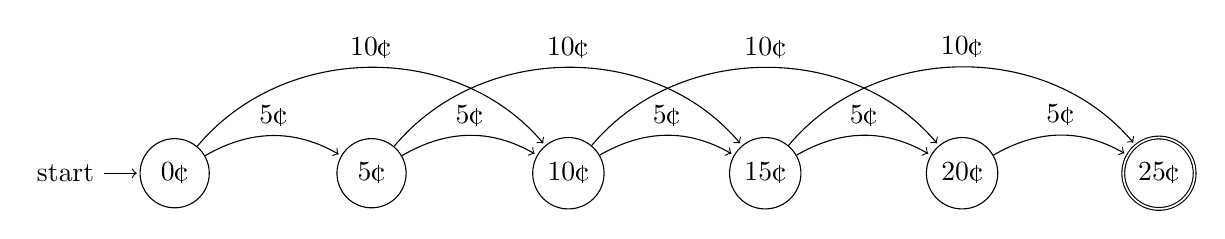
\begin{tikzpicture}[shorten >=1pt, node distance=2.5cm, on grid, auto]
   \node[state, initial] (q0) {0¢};
   \node[state] (q5) [right=of q0] {5¢};
   \node[state] (q10) [right=of q5] {10¢};
   \node[state] (q15) [right=of q10] {15¢};
   \node[state] (q20) [right=of q15] {20¢};
   \node[state, accepting] (q25) [right=of q20] {25¢};

    \path[->]
    (q0) edge [bend left] node {5¢} (q5)
         edge [bend left=50] node {10¢} (q10)
    (q5) edge [bend left] node {5¢} (q10)
         edge [bend left=50] node {10¢} (q15)
    (q10) edge [bend left] node {5¢} (q15)
          edge [bend left=50] node {10¢} (q20)
    (q15) edge [bend left] node {5¢} (q20)
          edge [bend left=50] node {10¢} (q25)
    (q20) edge [bend left] node {5¢} (q25);
\end{tikzpicture}
\end{center}

\paragraph*{Variable Names}

\textbf{Specification:} In defining a programming language, valid variable names should:
\begin{itemize}
    \item Start with a letter (\(\ell = a, b, c, \dots, z\)).
    \item Be followed by any combination of letters (\(\ell\)) or digits (\(d = 0,1,2,\dots,9\)).
    \item End with a terminal symbol (\(t\), e.g., \(t = ;\)).
\end{itemize}

\textbf{Automaton:} Accepted words follow the pattern:
\[
\ell (\ell + d)^* t
\]

\newpage

\paragraph*{Turnstile}

\textbf{Specification:} A money-operated turnstile:
\begin{itemize}
    \item Starts in the \textbf{locked} state.
    \item From \textbf{locked}:
    \begin{itemize}
        \item A \textbf{push} (\( u \)) keeps it \textbf{locked}.
        \item A \textbf{pay} (\( p \)) moves it to the \textbf{unlocked} state.
    \end{itemize}
    \item From \textbf{unlocked}:
    \begin{itemize}
        \item A \textbf{pay} (\( p \)) keeps it \textbf{unlocked}.
        \item A \textbf{push} (\( u \)) moves it back to \textbf{locked}.
    \end{itemize}
    \item The \textbf{unlocked} state is the accepting state.
\end{itemize}

\begin{center}
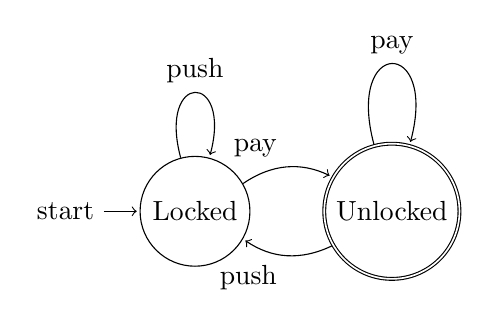
\begin{tikzpicture}[shorten >=1pt, node distance=2.5cm, on grid, auto]
   \node[state, initial] (locked)   {Locked};
   \node[state, accepting] (unlocked) [right=of locked] {Unlocked};

    \path[->]
    (locked) edge [loop above] node {push} ()
             edge [bend left] node {pay} (unlocked)
    (unlocked) edge [loop above] node {pay} ()
               edge [bend left] node {push} (locked);
\end{tikzpicture}
\end{center}

\subsubsection{Homework}

\paragraph*{Exercise: Characterizing Accepted Words}

Characterize all accepted words (i.e., describe exactly those words that are recognized).

The vending machine automaton accepts words consisting of payments in increments of 5 and 10 cents, reaching exactly 25 cents. The accepted words follow the pattern:

\[
(10 + 5)^*
\]

subject to the constraint that the sum of the numbers in the sequence equals 25.

\paragraph*{Exercise: Turnstile Regular Expression}

Characterize all accepted words and describe them using a regular expression.

The turnstile automaton can be characterized by the following regular expression:

\[
(p + u p)^* p (p + u p)^*
\]

where:
\begin{itemize}
    \item \( p \) represents a \textbf{pay} action.
    \item \( u \) represents a \textbf{push} action.
    \item \( p^* \) means zero or more additional \textbf{pay} actions while the turnstile remains open.
    \item The entire sequence can repeat any number of times.
\end{itemize}

\paragraph*{Example Accepted Words}
\begin{align*}
    & p &\quad \text{(Pay once, unlocks, and stays open)} \\
    & p p &\quad \text{(Pay twice, remains unlocked)} \\
    & p u p &\quad \text{(Pay, push to lock, then pay again to unlock)} \\
    & p p u p p p &\quad \text{(Multiple pays, a push to lock, then more pays)} \\
    & u p u p u p &\quad \text{(Invalid pushes in locked state, followed by pays to unlock)}
\end{align*}

\paragraph*{Exercise: Word Classification in Languages}

Determine for the following words if they are contained in \(L_1\), \(L_2\), or \(L_3\).

Here, based on the descriptions given later in the report:
\begin{itemize}
    \item \(L_1\) is the set of words that contain the substring ``01''.
    \item \(L_2\) is the set of words whose lengths are powers of two.
    \item \(L_3\) is the set of words with an equal number of 0s and 1s.
\end{itemize}

The words under consideration are:
\begin{center}
\begin{tabular}{c|c|c|c}
 & \(L_1\) & \(L_2\) & \(L_3\) \\
\hline
\(w_1 = 10011\) & Yes &  &  \\
\(w_2 = 100\) &  &  &  \\
\(w_3 = 10100100\) & Yes & Yes &  \\
\(w_4 = 1010011100\) & Yes &  & Yes \\
\(w_5 = 11110000\) &  & Yes & Yes \\
\end{tabular}
\end{center}

\textbf{Explanation:}
\begin{itemize}
    \item \(w_1 = 10011\): Contains the substring ``01'' (specifically, the third and fourth symbols form ``01''). Its length is 5 (not a power of two), and it has 3 ones versus 2 zeros.
    \item \(w_2 = 100\): Does not contain the substring ``01'' (the pairs are ``10'' and ``00''), its length is 3 (not a power of two), and it has 1 one and 2 zeros.
    \item \(w_3 = 10100100\): Contains ``01'' (for example, the second and third symbols form ``01''); its length is 8 (which is \(2^3\)); however, it has 3 ones and 5 zeros.
    \item \(w_4 = 1010011100\): Contains ``01'' (e.g., the first occurrence between the first and second symbols or elsewhere); its length is 10 (not a power of two); and it has 5 ones and 5 zeros.
    \item \(w_5 = 11110000\): Does not contain the substring ``01'' (the transition from 1s to 0s gives ``10'' rather than ``01''); its length is 8 (a power of two); and it has 4 ones and 4 zeros.
\end{itemize}

\paragraph*{Exercise: DFA Run Acceptance}

Consider the DFA from above (see \href{https://hackmd.io/_uploads/ByLSmw_tyl.jpg}{dfa\_example}). Consider the paths corresponding to the words \(w_1 = 0010\), \(w_2 = 1101\), and \(w_3 = 1100\). For which of these words does their run end in the accepting state?

\textbf{Definition.} We call
\[
L(\mathcal{A}) := \{w \in \Sigma^* \; | \; \text{The run for \(w\) in \(\mathcal{A}\) ends in some \(q \in F\)} \}
\]
the language \textit{accepted} by \(\mathcal{A}\).

\newpage

\textbf{Answer:} After tracing the transitions in the given DFA, we find that:
\begin{itemize}
    \item For \(w_1 = 0010\), the run ends in a non-accepting state.
    \item For \(w_2 = 1101\), the run ends in a non-accepting state.
    \item For \(w_3 = 1100\), the run ends in an accepting state.
\end{itemize}

One plausible interpretation (consistent with common examples such as a DFA for determining divisibility by 3 or for ensuring an even number of 1s) shows that only \(w_3\) meets the acceptance condition, while \(w_1\) and \(w_2\) do not.

\subsubsection*{Summary of Week 1}

Finite automata are abstract machines used to recognize regular languages, which can be fully described using finite-state transitions. This chapter explores deterministic finite automata (DFAs) and nondeterministic finite automata (NFAs), demonstrating that NFAs, despite their flexibility, recognize the same class of languages as DFAs.

A key distinction between the two is that DFAs have a single active state at any time, whereas NFAs may simultaneously exist in multiple states. While NFAs simplify language representation, they can always be converted into equivalent DFAs through an algorithmic transformation.

An important extension of NFAs allows transitions on the empty string, further enhancing their expressiveness while still recognizing only regular languages. These \(\varepsilon\)-NFAs will later play a crucial role in proving the equivalence of finite automata and regular expressions.

The chapter also introduces an applied perspective on finite automata through a real-world example: electronic money protocols. By modeling interactions between a bank, a store, and a customer as finite automata, the protocol’s correctness and potential fraud vulnerabilities can be analyzed. The study concludes with constructing a product automaton to validate interactions, ensuring that transactions occur as intended while preventing unauthorized duplication or cancellation of funds.

\subsubsection{Conclusion}

Deterministic Finite Automata (DFAs) are a fundamental concept in automata theory, providing a mathematical model for recognizing patterns in strings. A DFA is defined as a tuple \(\mathcal{A} = (Q, \Sigma, \delta, q_0, F)\), where \(Q\) is a finite set of states, \(\Sigma\) is an input alphabet, \(\delta\) is the transition function mapping states and symbols to new states, \(q_0\) is the initial state, and \(F\) is the set of accepting states. DFAs process input strings deterministically, meaning that for every state and input symbol, there is exactly one transition.

Formal languages are sets of words over an alphabet \(\Sigma\). The set of all possible words is denoted \(\Sigma^*\), which includes the empty word \(\varepsilon\). The length of a word \(w\) is written as \(|w|\), and the occurrence of a symbol \(a\) in \(w\) is denoted \(|w|_a\). Example languages include \(L_1\), which contains words with the substring “01,” \(L_2\), which consists of words whose lengths are powers of two, and \(L_3\), which contains words with an equal number of 0s and 1s.

DFAs determine if a word belongs to a language by processing transitions. If the final state is in \(F\), the word is accepted; otherwise, it is rejected.

\newpage

\subsection{Week 2: DFA Implementation in Python}

\subsubsection{Introduction}
In this homework, we explore the implementation of deterministic finite automata (DFAs) in Python. We will go beyond the simple graphical representation of DFAs and build them using Python types.

\subsubsection{Readings}
\paragraph*{Chapter 2.2.4}
A \textbf{Deterministic Finite Automaton (DFA)} is a formal model of computation that processes input sequences while maintaining a single, well-defined state at any given time. The term "deterministic" means that for each input symbol, the automaton transitions to exactly one state.


\subsubsection{Homework}

\paragraph*{Implementing DFAs in Python}
We will implement the following DFAs in Python using this \texttt{DFA} class:

\begin{verbatim}
class DFA:

    def __init__(self, Q, Sigma, delta, q0, F):
        self.Q = Q  # Set of states
        self.Sigma = Sigma  # Alphabet
        self.delta = delta  # Transition function (dict)
        self.q0 = q0  # Initial state
        self.F = F  # Set of accepting states

    def __repr__(self):
        return f"DFA({self.Q},\n\t{self.Sigma},\n\t{self.delta},
                      \n\t{self.q0},\n\t{self.F})"

    def run(self, w):
        current_state = self.q0  # Start at initial state
        loop = 0
        for symbol in w:
            loop += 1
            if symbol not in self.Sigma:
                return False  # Reject if symbol is not in the alphabet
            if (current_state, symbol) not in self.delta:
                return False  # Reject if there's no valid transition
            current_state = self.delta[(current_state, symbol)]  # Move to next state
        
        return current_state in self.F  # Accept if final state is in F
\end{verbatim}

\newpage

\paragraph*{Exercise 1: Word Processing with DFAs}
\begin{center}
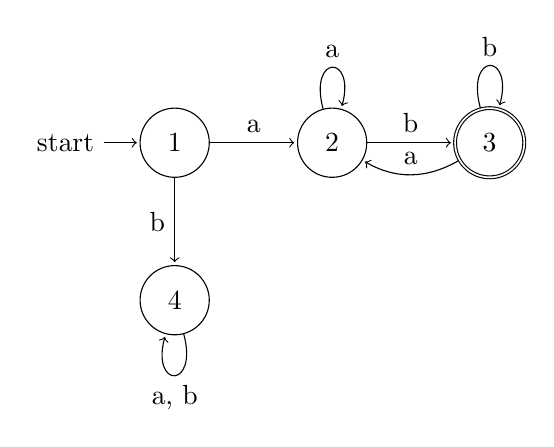
\begin{tikzpicture}[shorten >=1pt, node distance=2cm, on grid, auto] 
   \node[state, initial] (q_1) {1}; 
   \node[state] (q_2) [right=of q_1] {2}; 
   \node[state, accepting] (q_3) [right=of q_2] {3}; 
   \node[state] (q_4) [below=of q_1] {4};

   \path[->] 
    (q_1) edge [above] node {a} (q_2)
          edge [left] node {b} (q_4)
    (q_2) edge [loop above] node {a} ()
          edge [above] node {b} (q_3)
    (q_3) edge [bend left, above] node {a} (q_2)
          edge [loop above] node {b} ()
    (q_4) edge [loop below] node {a, b} (); 
\end{tikzpicture}

\textit{Automaton \(\mathcal{A}_1\)}
\end{center}

\begin{center}
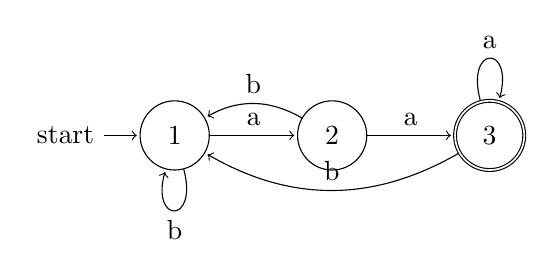
\begin{tikzpicture}[shorten >=1pt, node distance=2cm, on grid, auto] 
   \node[state, initial] (q_1) {1}; 
   \node[state] (q_2) [right=of q_1] {2}; 
   \node[state, accepting] (q_3) [right=of q_2] {3}; 

   \path[->] 
    (q_1) edge [above] node {a} (q_2)
          edge [loop below] node {b} ()
    (q_2) edge [above] node {a} (q_3)
          edge [bend right, above] node {b} (q_1)
    (q_3) edge [loop above] node {a} ()
          edge [bend left, above] node {b} (q_1);
\end{tikzpicture}

\textit{Automaton \(\mathcal{A}_2\)}
\end{center}

Here is how we initialize the DFAs in Python:

\begin{verbatim}
    # DFA A1
    Q = {1,2,3,4}
    Sigma = {'a','b'}
    delta = {(1,'a'):2, (1,'b'):4, (2,'a'):2, (2,'b'):3, 
             (3,'a'):2, (3,'b'):2, (4,'a'):4, (4,'b'):4}
    q0 = 1
    F = {3}
    A1 = dfa.DFA(Q, Sigma, delta, q0, F)
    
    # DFA A2
    Q = {1,2,3}
    Sigma = {'a','b'}
    delta = {(1,'a'):2, (1,'b'):1, (2,'a'):3, (2,'b'):1,
             (3,'a'):3, (3,'b'):1}
    q0 = 1
    F = {3}
    A2 = dfa.DFA(Q, Sigma, delta, q0, F)
\end{verbatim}

\newpage

\paragraph*{Constructing the Complement DFA}
To construct an automaton \(A_0\) that accepts exactly the words that \(A\) refuses and vice versa we can simply swap the accepting states with the previously non-accepting states.

\begin{center}
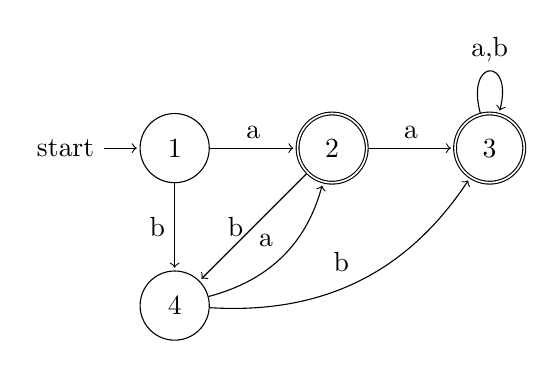
\begin{tikzpicture}[shorten >=1pt, node distance=2cm, on grid, auto] 
    \node[state, initial] (q_1) {1}; 
    \node[state, accepting] (q_2) [right=of q_1] {2}; 
    \node[state, accepting] (q_3) [right=of q_2] {3}; 
    \node[state] (q_4) [below=of q_1] {4};

    \path[->] 
        (q_1) edge [above] node {a} (q_2)
              edge [left] node {b} (q_4)
        (q_2) edge [above] node {a} (q_3)
              edge [left] node {b} (q_4)
        (q_3) edge [loop above] node {a,b} ()
        (q_4) edge [bend right] node {a} (q_2)
              edge [bend right] node {b} (q_3);
\end{tikzpicture}
\end{center}

We can represent this operation with a \texttt{refuse()} function in Python:

\begin{verbatim}
def refuse(A):
    """Constructs a DFA A0 that accepts exactly the words that A refuses and vice versa."""
    Q0 = A.Q
    Sigma0 = A.Sigma
    delta0 = A.delta
    q0_0 = A.q0
    F0 = Q0 - A.F  # Complement of the accepting states

    return dfa.DFA(Q0, Sigma0, delta0, q0_0, F0)
\end{verbatim}

\paragraph*{Exercise 2.4.4}
\textbf{(a) DFA for strings ending in 00}

\begin{center}
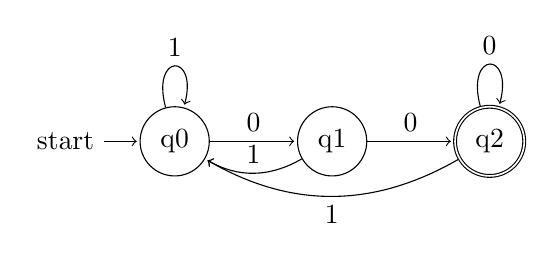
\begin{tikzpicture}[shorten >=1pt, node distance=2cm, on grid, auto]
    \node[state, initial] (q0) {q0};
    \node[state] (q1) [right=of q0] {q1};
    \node[state, accepting] (q2) [right=of q1] {q2};

    \path[->] 
        (q0) edge [loop above] node {1} ()
             edge [above] node {0} (q1)
        (q1) edge [above] node {0} (q2)
             edge [bend left, above] node {1} (q0)
        (q2) edge [loop above] node {0} ()
             edge [bend left] node {1} (q0);
\end{tikzpicture}
\end{center}

\textbf{(b) DFA for strings containing 000 as a substring}

\begin{center}
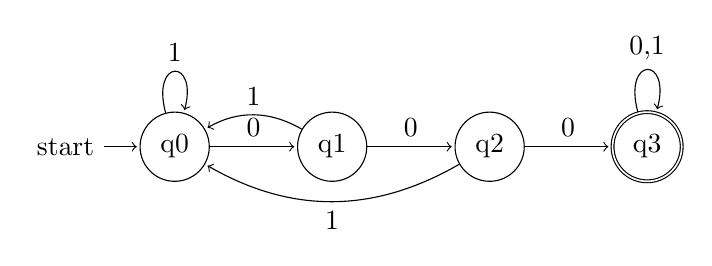
\begin{tikzpicture}[shorten >=1pt, node distance=2cm, on grid, auto]
    \node[state, initial] (q0) {q0};
    \node[state] (q1) [right=of q0] {q1};
    \node[state] (q2) [right=of q1] {q2};
    \node[state, accepting] (q3) [right=of q2] {q3};

    \path[->]
        (q0) edge [loop above] node {1} ()
             edge [above] node {0} (q1)
        (q1) edge [above] node {0} (q2)
             edge [bend right, above] node {1} (q0)
        (q2) edge [above] node {0} (q3)
             edge [bend left, below] node {1} (q0)
        (q3) edge [loop above] node {0,1} (); 
\end{tikzpicture}
\end{center}

\textbf{(c) DFA for strings containing 011 as a substring}

\begin{center}
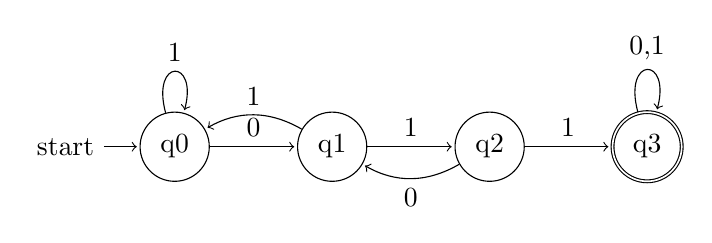
\begin{tikzpicture}[shorten >=1pt, node distance=2cm, on grid, auto]
    \node[state, initial] (q0) {q0};
    \node[state] (q1) [right=of q0] {q1};
    \node[state] (q2) [right=of q1] {q2};
    \node[state, accepting] (q3) [right=of q2] {q3};

    \path[->]
        (q0) edge [loop above] node {1} ()
             edge [above] node {0} (q1)
        (q1) edge [above] node {1} (q2)
             edge [bend right, above] node {1} (q0)
        (q2) edge [above] node {1} (q3)
             edge [bend left, below] node {0} (q1)
        (q3) edge [loop above] node {0,1} (); 
\end{tikzpicture}
\end{center}

\newpage

\subsubsection{Conclusion}
A \textbf{Deterministic Finite Automaton (DFA)} is a theoretical computational model used to recognize formal languages. A DFA consists of a finite set of states \( Q \), an input alphabet \( \Sigma \), a transition function \( \delta: Q \times \Sigma \to Q \), a start state \( q_0 \), and a set of accepting states \( F \). The machine processes strings sequentially, transitioning between states according to \( \delta \). If, after consuming the entire string, the DFA ends in an accepting state, the input is accepted; otherwise, it is rejected.

\newpage

\subsection{Week 3: DFAs and NFAs}

\subsubsection{Introduction}
This week we covered ways to combine automata. We focused on the set theory used in the combination as well as some notation.  
Lastly, we introduced Nondeterministic Finite Automatas, or NFAs.

\subsubsection{Homework}

\paragraph*{Extended Transition Functions}
\textbf{Brief summary of the question:}
Given the two DFAs below:
\begin{itemize}
  \item Compute the extended transition functions 
    \(\hat\delta^{(1)}(1,\,abaa)\) and \(\hat\delta^{(2)}(1,\,abba)\), 
    showing all steps.
  \item Describe the language accepted by each automaton.
\end{itemize}

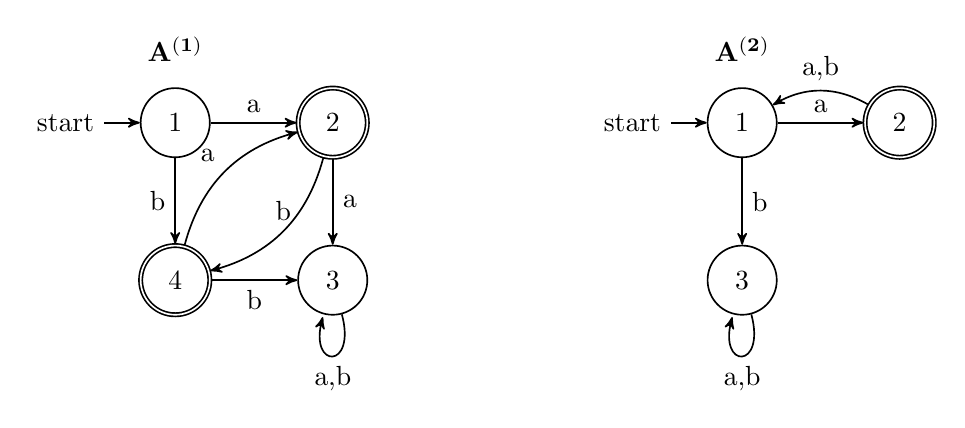
\begin{tikzpicture}[->, >=stealth', auto, node distance=2.0cm, semithick]
  % First automaton A^{(1)}
  \begin{scope}
    \node[state, initial] (1a) {1};
    \node[state, accepting, right of=1a] (2a) {2};
    \node[state, below of=2a] (3a) {3};
    \node[state, accepting, below of=1a] (4a) {4};

    \path
      (1a) edge              node {a} (2a)
            edge[left]       node {b} (4a)
      (2a) edge              node {a} (3a)
            edge[bend left,above]  node {b} (4a)
      (4a) edge[bend left]  node {a} (2a)
            edge[below]            node {b} (3a)
      (3a) edge[loop below] node {a,b} ();
    \draw node at (1a.north) [above=0.2cm] {\(\mathbf{A^{(1)}}\)};
  \end{scope}

  % Second automaton A^{(2)}
  \begin{scope}[xshift=7.2cm]
    \node[state, initial] (1b) {1};
    \node[state, accepting, right of=1b] (2b) {2};
    \node[state, below of=1b] (3b) {3};

    \path
      (1b) edge              node {a} (2b)
            edge              node {b} (3b)
      (2b) edge[bend right, above]  node {a,b} (1b)
      (3b) edge[loop below]  node {a,b} ();
    \draw node at (1b.north) [above=0.2cm] {\(\mathbf{A^{(2)}}\)};
  \end{scope}
\end{tikzpicture}

\[
  L\bigl(A^{(1)}\bigr) = \{\,w\in\{a,b\}^+\mid\text{no two consecutive symbols are the same}\},
\]
\[
  L\bigl(A^{(2)}\bigr) = a\,((a\mid b)\,a)^* 
    = \{\,w\in\{a,b\}^*\mid\text{$w$ has odd length, starts with $a$, and every odd position is $a$}\}.
\]

\[
  \hat{\delta}^{(1)}(1,\,abaa)=3,
  \quad
  \hat{\delta}^{(2)}(1,\,abba)=3.
\]

\newpage

\paragraph*{Intersubsection Automaton for \(A^{(1)}\) and \(A^{(2)}\)}
We form the product automaton
\[
  A = (Q^{(1)}\times Q^{(2)},\,\Sigma,\,\delta,\,(q_0^{(1)},q_0^{(2)}),\,F^{(1)}\times F^{(2)}),
\]
where
\[
  Q^{(1)}=\{1,2,3,4\},\;
  Q^{(2)}=\{1,2,3\},\;
  \Sigma=\{a,b\},
\]
\(\delta((p,q),x)=(\delta^{(1)}(p,x),\delta^{(2)}(q,x))\),
and accepting states \(F^{(1)}\times F^{(2)}\).

\begin{center}
  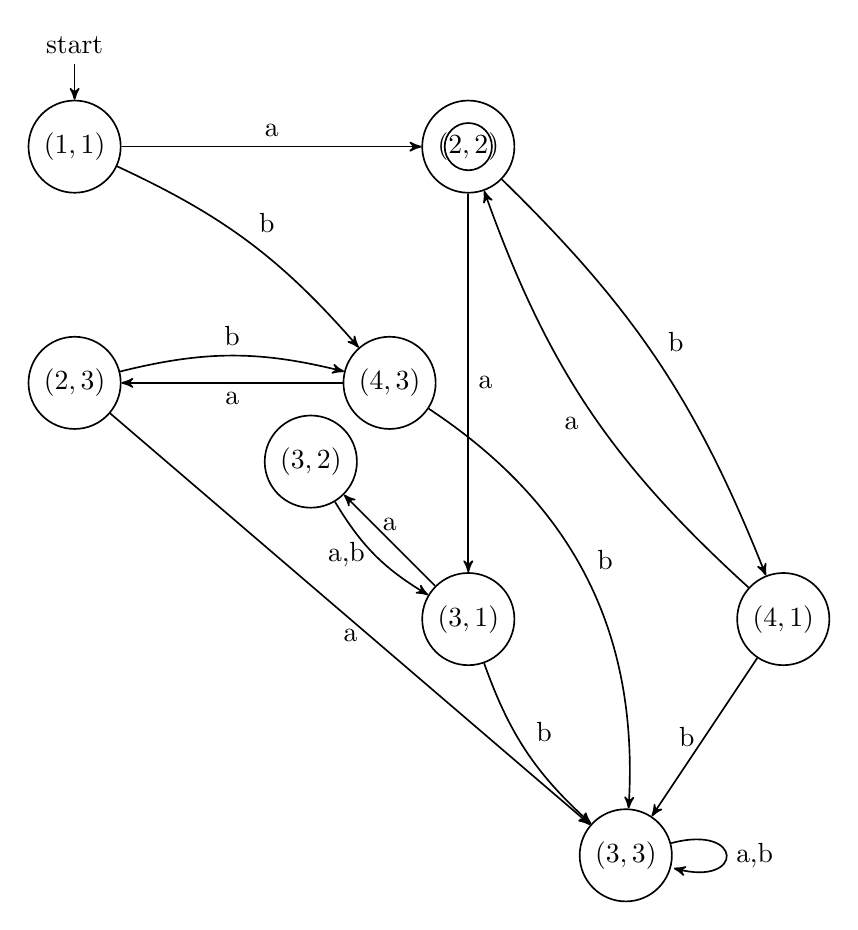
\begin{tikzpicture}[->,>=stealth',auto,semithick]
    % ------------------------------------------------------------------
    %                             NODES
    % ------------------------------------------------------------------
    % top row
    \node[state,initial above] (11) at (0,0)        {\((1,1)\)};
    \node[state]               (22) at (5,0)        {\((2,2)\)};
    % second row
    \node[state]               (23) at (0,-3)       {\((2,3)\)};
    \node[state]               (43) at (4,-3)       {\((4,3)\)};
    % third row
    \node[state]               (31) at (5,-6)       {\((3,1)\)};
    \node[state]               (41) at (9,-6)       {\((4,1)\)};
    % bottom row
    \node[state]               (32) at (3,-4)       {\((3,2)\)};
    \node[state]               (33) at (7,-9)       {\((3,3)\)};
  
    % mark (2,2) as accepting
    \draw (22) circle [draw=black,very thick,x radius=0.30cm,y radius=0.30cm];
  
    % ------------------------------------------------------------------
    %                             EDGES
    % ------------------------------------------------------------------
    \path
      % from (1,1)
      (11) edge [above]             node {a} (22)
           edge [bend left=12]      node {b} (43)
      % from (2,2)
      (22) edge [right]             node {a} (31)
           edge [bend left=12]      node {b} (41)
      % from (4,3)
      (43) edge [left, below]              node {a} (23)
           edge [bend left]             node {b} (33)
      % from (3,1)
      (31) edge [below left, above]        node {a} (32)
           edge [bend right=14]     node {b} (33)
      % from (4,1)
      (41) edge [bend left=14]      node {a} (22)
           edge [left]              node {b} (33)
      % from (2,3)
      (23) edge [below]             node {a} (33)
           edge [bend left=14,above] node {b} (43)
      % from (3,3)
      (33) edge [loop right]        node {a,b} ()
      % from (3,2)
      (32) edge [bend right=14, below, left] node {a,b} (31);
  \end{tikzpicture}
  
\end{center}

\paragraph*{Why \(L(A)=L(A^{(1)})\cap L(A^{(2)})\)?}
\(A\) simulates both in parallel and accepts iff both coordinates are accepting.

\paragraph*{Changing to Obtain Union}
Use the same transitions but set
\[
  F' = (F^{(1)}\times Q^{(2)})\;\cup\;(Q^{(1)}\times F^{(2)}),
\]
so \(L(A')=L(A^{(1)})\cup L(A^{(2)})\).

\subsubsection*{Exercise 2.2.7}
\textbf{Claim.} If \(\delta(q,a)=q\) for all \(a\), then \(\delta(q,w)=q\) for any \(w\).

\textbf{Proof (by induction):}
Base: \(\delta(q,\varepsilon)=q\).  
Step: \(\delta(q,xa)=\delta(\delta(q,x),a)=\delta(q,a)=q\).

\subsubsection{Readings}

\paragraph*{Chapter 2.3}
The extended transition function for an NFA,
\[
  \hat{\delta}(q,\varepsilon)=\{q\},\quad
  \hat{\delta}(q,\,xa)=\bigcup_{p\in\hat{\delta}(q,x)}\delta(p,a),
\]
captures nondeterminism.  The subset construction converts an NFA \(N\) into a DFA \(D\) whose states are subsets of \(N\)’s states, preserving \(L(D)=L(N)\).

\subsubsection{Conclusion}
Throughout these problems and readings, we deepened our understanding of DFAs and NFAs: extended transition functions, intersubsection/union constructions, and the subset construction proving NFA–DFA equivalence.

\textbf{Interesting question: Maximal Blow-Up in the Subset Construction.}\\
Describe an \(n\)-state NFA forcing all \(2^n\) subsets to appear in its equivalent DFA and prove minimality.

\subsection{Week 4: Determinization}

\subsubsection{Introduction}
In this report, we explore fundamental aspects of both deterministic and nondeterministic finite automata (DFAs and NFAs), including extended transition functions, product automaton construction for intersubsection, and state modifications for union. We further demonstrate the subset construction to establish the equivalence of NFAs and DFAs, showcasing the broad utility of these automata concepts in both theoretical and practical contexts.

\subsubsection{Homework}

\paragraph*{Homework 1}

Let \(\mathcal{A} = (Q, \Sigma, \delta: Q \times \Sigma \to Q, q_0, F)\) be a DFA. Explain in what way you can view \(\mathcal{A}\) as an NFA by doing the following:
\begin{enumerate}
\item Let \(\mathcal{A}\) denote the following DFA:
\[
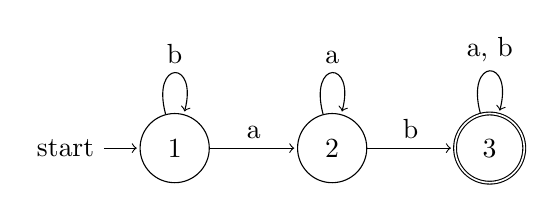
\begin{tikzpicture}[shorten >=1pt,node distance=2.0cm,on grid,auto]
   \node[state, initial] (q1) {1};
   \node[state] (q2) [right=of q1] {2};
   \node[state, accepting] (q3) [right=of q2] {3};

   \path[->]
   (q1) edge[loop above] node {b} (q1)
        edge node {a} (q2)
   (q2) edge[loop above] node {a} (q2)
        edge node {b} (q3)
   (q3) edge[loop above] node {a, b} (q3);
\end{tikzpicture}
\]

Here:
\[
\begin{aligned}
Q &= \{1,2,3\}, \quad \Sigma = \{a,b\}, \\
q_0 &= 1, \quad F = \{3\}, \\
\delta(1,a) &= 2,\ \delta(1,b) = 1, \\
\delta(2,a) &= 2,\ \delta(2,b) = 3, \\
\delta(3,a) &= 3,\ \delta(3,b) = 3.
\end{aligned}
\]
Explain how you can understand \(\mathcal{A}\) also as an NFA.

\item More generally, let \(\mathcal{A} = (Q, \Sigma, \delta: Q \times \Sigma \to Q, q_0, F)\) be a DFA. Define an NFA
\[
\mathcal{A}' = (Q', \Sigma, \delta': Q' \times \Sigma \to \mathcal{P}(Q'), q_0', F')
\]
such that \(L(\mathcal{A}) = L(\mathcal{A}')\).

\item Justify why your construction satisfies the desired condition.
\end{enumerate}

\newpage

\paragraph*{Solutions}
\paragraph{1) Viewing the Example DFA as an NFA}  
A deterministic finite automaton (DFA) can be seen as a special case of a nondeterministic finite automaton (NFA) by interpreting its transition function in the following way: in an NFA, the transition function 
\[
\delta': Q \times \Sigma \to \mathcal{P}(Q)
\]
produces \emph{sets} of possible next states. In a DFA, however, for each state \(q\) and input symbol \(a\), there is exactly one next state \(\delta(q,a)\). To view the DFA as an NFA, we simply set:
\[
\delta'(q,a) = \{\delta(q,a)\}.
\]
Hence, each transition in the original DFA becomes a transition to a \emph{singleton set} in the NFA, preserving the recognized language because no extra nondeterminism is introduced.

\paragraph{2) General Construction from a DFA to an NFA}  
Given any DFA 
\(\mathcal{A} = (Q, \Sigma, \delta, q_0, F)\),
define an NFA
\(\mathcal{A}' = (Q', \Sigma, \delta', q_0', F')\) by:
\[
\begin{aligned}
Q' &= Q,\\
q_0' &= q_0,\\
F' &= F,\\
\delta'(q,a) &= \{\delta(q,a)\} \quad\text{for all }q\in Q,\ a\in\Sigma.
\end{aligned}
\]

\paragraph{3) Why \(L(\mathcal{A}) = L(\mathcal{A}')\)?}  
Because each step in the DFA corresponds to a unique singleton transition in the NFA:
\begin{itemize}
  \item If a string \(w\) is accepted by the DFA, the identical path exists in the NFA.
  \item If a string \(w\) is rejected by the DFA, no path in the NFA leads to acceptance.
\end{itemize}
Thus the two automata recognize the same language.

\paragraph*{Homework 2}
\begin{enumerate}
  \item Describe in words the language \(L(\mathcal{A})\) accepted by the NFA \(\mathcal{A}\) pictured below.
  \item Specify the automaton \(\mathcal{A}\) formally as \((Q,\Sigma,\delta,q_0,F)\).
  \item Using the extended transition function \(\hat{\delta}\), compute \(\hat{\delta}(q_0,10110)\) step by step.
  \item Find \emph{all} paths in \(\mathcal{A}\) for \(v=1100\) and \(w=1010\); represent each set of paths.
  \item Construct the determinization \(\mathcal{A}^D\) (power-set automaton) of \(\mathcal{A}\).
  \item Verify \(L(\mathcal{A}) = L(\mathcal{A}^D)\). Is there a smaller DFA for the same language?
\end{enumerate}

\newpage

\paragraph*{Solutions}
Below is the NFA \(\mathcal{A}\):

\begin{center}
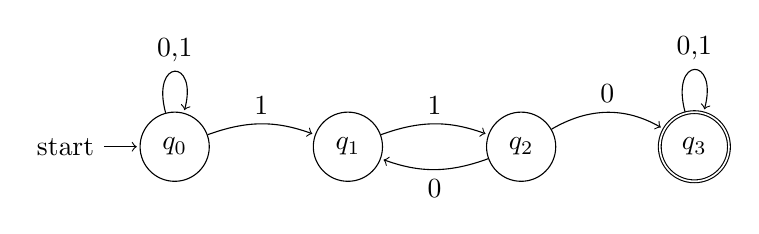
\begin{tikzpicture}[shorten >=1pt,node distance=2.2cm,on grid,auto]
   \node[state, initial] (q0) {\(q_0\)};
   \node[state] (q1) [right=of q0] {\(q_1\)};
   \node[state] (q2) [right=of q1] {\(q_2\)};
   \node[state, accepting] (q3) [right=of q2] {\(q_3\)};

   \path[->]
   (q0) edge[loop above] node {0,1} (q0)
        edge[bend left=20] node {1} (q1)
   (q1) edge[bend left=20] node {1} (q2)
   (q2) edge[bend left=20] node {0} (q1)
        edge[bend left=30] node {0} (q3)
   (q3) edge[loop above] node {0,1} (q3);
\end{tikzpicture}
\end{center}

\paragraph{1) Language Description}  
\(\mathcal{A}\) accepts exactly those binary strings that can nondeterministically traverse  
\(q_0\to q_1\to q_2\) on two 1’s and then take a 0 to \(q_3\), after which any symbols are allowed.

\paragraph{2) Formal Specification}  
\[
\mathcal{A} = (Q,\Sigma,\delta,q_0,F),
\quad
Q=\{q_0,q_1,q_2,q_3\},\;\Sigma=\{0,1\},\;F=\{q_3\},
\]
with
\[
\begin{aligned}
\delta(q_0,0)&=\{q_0\},\;\delta(q_0,1)=\{q_0,q_1\},\\
\delta(q_1,1)&=\{q_2\},\;\delta(q_1,0)=\varnothing,\\
\delta(q_2,0)&=\{q_1,q_3\},\;\delta(q_2,1)=\varnothing,\\
\delta(q_3,a)&=\{q_3\}\quad(a\in\{0,1\}).
\end{aligned}
\]

\paragraph{3) Extended Transition on 10110}  
\(\hat{\delta}(q_0,\varepsilon)=\{q_0\}\),  
\(\hat{\delta}(q_0,1)=\{q_0,q_1\}\),  
\(\hat{\delta}(\{q_0,q_1\},0)=\{q_0\}\),  
\(\hat{\delta}(\{q_0\},1)=\{q_0,q_1\}\),  
\(\hat{\delta}(\{q_0,q_1\},1)=\{q_0,q_1,q_2\}\).

\paragraph{4) All Paths for 1100 and 1010}  
Branches arise at each nondeterministic choice; any accepting path must include  
\(q_0\xrightarrow{1}q_1\xrightarrow{1}q_2\xrightarrow{0}q_3\).

% should be in the format from class, showing branche, 2 words may have different paths

\paragraph{5) Determinization (Power-Set)}  
\[
Q^D=\mathcal{P}(Q),\;
q_0^D=\{q_0\},\;
F^D=\{S:S\cap\{q_3\}\neq\varnothing\},\;
\delta^D(S,a)=\bigcup_{s\in S}\delta(s,a).
\]

% write explicetly for the given automata ubove

\paragraph{6) Verification \& Minimization}  
By construction \(L(\mathcal{A}^D)=L(\mathcal{A})\). The resulting DFA can then be minimized via standard algorithms.

\subsubsection{Conclusion}
By viewing any DFA as an NFA with singleton transitions and applying the subset (powerset) construction, we have shown that NFAs and DFAs recognize exactly the same class of languages.  This determinization process not only establishes the theoretical equivalence of nondeterministic and deterministic finite automata but also provides a concrete algorithm for converting an NFA into an equivalent DFA, reinforcing the practical utility of these foundational automata concepts.

\newpage

\subsection{Week 5: Equivalence and Minimization of Automata}

\subsubsection{Introduction}
This report focuses on Equivalence and Minimization of Automata, covering the process of determining whether two different DFA representations define the same language and how to construct the smallest possible DFA that accepts a given regular language. The table‐filling algorithm is introduced as a systematic way to check equivalence of states within a DFA by distinguishing them through input strings. This allows us to merge equivalent states, reducing the number of states while preserving language recognition. We also examine the uniqueness of the minimal DFA and its theoretical guarantees. Finally, the report discusses the complexity of these procedures and their implications for automata design.

\subsubsection{Readings}

\paragraph*{Chapter 4.4 – Equivalence and Minimization of Automata}
Chapter 4.4 covers the equivalence and minimization of automata, focusing on the problem of determining whether two descriptions of regular languages define the same language. The chapter introduces the table‐filling algorithm, a method to determine when two states of a DFA are equivalent by examining how they transition on different input strings. If two states lead to the same accepting or rejecting states for all possible inputs, they are considered equivalent and can be merged into a single state. If not, they are distinguishable. This process allows us to construct a minimal DFA, the smallest DFA that accepts a given language. The minimization process follows a structured approach:
\begin{enumerate}
  \item Eliminate unreachable states.
  \item Partition the remaining states into equivalence classes.
  \item Construct a new DFA where each equivalence class represents a single state.
\end{enumerate}
A key result is that the minimal DFA is unique up to renaming of states. The chapter also explores the complexity of minimization, showing that the table‐filling algorithm runs in \(O(n^2)\) time. Additionally, it presents an alternative perspective on DFA equivalence testing by constructing a combined DFA from two automata and checking equivalence of their start states. The final part discusses NFA minimization and its inherent difficulties compared to DFAs, highlighting limitations of direct state‐equivalence methods for NFAs.

\subsubsection{Homework}
\textbf{Note:} The following exercises test understanding of state equivalence, DFA minimization, and nonregularity proofs.

\paragraph*{Exercise 3.2.1}
Here is the DFA’s transition table:
\[
\begin{array}{c|cc}
     &0&1\\\hline
\to q_1 & q_2 & q_1\\
      q_2 & q_3 & q_1\\
*\,q_3 & q_3 & q_2
\end{array}
\]
\paragraph{(a) \(R_{ij}^{(0)}\)}
\[
\begin{array}{c|ccc}
R_{ij}^{(0)} & j=1 & j=2 & j=3\\\hline
i=1 & \varepsilon\cup1 & 0 & \varnothing\\
i=2 & 1 & \varnothing & 0\\
i=3 & \varnothing & 1 & \varepsilon\cup0
\end{array}
\]
\paragraph{(b) \(R_{ij}^{(1)}\)}
\[
\begin{array}{c|ccc}
R_{ij}^{(1)} & j=1 & j=2 & j=3\\\hline
i=1 & 1^* & 1^*0 & \varnothing\\
i=2 & 1^+ & 1^+0 & 0\\
i=3 & \varnothing & 1 & \varepsilon\cup0
\end{array}
\]
\paragraph{(c) \(R_{ij}^{(2)}\)}
\[
\begin{array}{c|ccc}
R_{ij}^{(2)} & j=1 & j=2 & j=3\\\hline
i=1 & 1^*\cup1^*0\,(0+1)^*\,1^+ 
      & 1^*0 
      & 1^*0\,(0+1)^*\,0\\
i=2 & 1^+ & 1^+0 & 0\\
i=3 & \varnothing & 1 & \varepsilon\cup0
\end{array}
\]
\paragraph{(d) Regular expression}
\[
(1 + 01)^*\,00\,(0 + 10)^*.
\]

\paragraph*{Exercise 3.2.2}
\[
\begin{array}{c|cc}
     &0&1\\\hline
\to q_1 & q_2 & q_3\\
      q_2 & q_1 & q_3\\
*\,q_3 & q_2 & q_1
\end{array}
\]
\paragraph{(a) \(R_{ij}^{(0)}\)}
\[
\begin{array}{c|ccc}
R_{ij}^{(0)} & j=1 & j=2 & j=3\\\hline
i=1 & \varepsilon & 0 & 1\\
i=2 & 0 & \varepsilon & 1\\
i=3 & 1 & 0 & \varepsilon
\end{array}
\]
\paragraph{(b) \(R_{ij}^{(1)}\)}
\[
\begin{array}{c|ccc}
R_{ij}^{(1)} & j=1 & j=2 & j=3\\\hline
i=1 & \varepsilon & 0 & 1\\
i=2 & 0 & \varepsilon\cup00 & 1\cup01\\
i=3 & 1 & 0\cup10 & \varepsilon\cup11
\end{array}
\]
\paragraph{(c) \(R_{13}^{(2)}\)}
\[
R_{13}^{(2)} = 1 \;\cup\;0\,(00)^*\,(1+01).
\]
\paragraph{(d) Regular expression}
\[
1 \;+\;0\,(00)^*\,(1+01).
\]

% i copied down the wrong problems, be sure to do 4.4.1 and 4.4.2 a and b, keep theese in though for extra credit

\paragraph*{Exercise 4.1.1}
Prove the following languages are not regular using the pumping lemma:

\paragraph{(a) \(\{0^n1^n\mid n\ge1\}\)}
\textbf{Proof.} Let \(p\) be the pumping length. Consider \(s=0^p1^p\). Any decomposition \(s=xyz\) with \(\lvert xy\rvert\le p\) forces \(y=0^k\) for some \(k\ge1\). Pumping down (\(i=0\)) yields \(0^{p-k}1^p\), which has fewer 0s than 1s, so \(0^{p-k}1^p\notin L\). Contradiction.

\paragraph{(b) Balanced parentheses}
\textbf{Proof.} Let \(p\) be the pumping length and take 
\[
s = (\underbrace{( \dots (}_{p}\underbrace{) \dots )}_{p}).
\]
Then \(\lvert s\rvert\ge p\), and any decomposition \(s=xyz\) with \(\lvert xy\rvert\le p\) has \(y\) consisting only of “(”. Pumping down removes some “(” while leaving all “)”, yielding an unbalanced string. Contradiction.

\paragraph{(c) \(\{0^n1\,0^n\mid n\ge1\}\)}
\textbf{Proof.} Let \(s=0^p1\,0^p\). Any \(s=xyz\) with \(\lvert xy\rvert\le p\) again gives \(y=0^k\). Pumping down produces \(0^{p-k}1\,0^p\), which no longer has equal numbers of leading and trailing 0s. Contradiction.

\paragraph{(d) \(\{0^n1^m2^n\mid n,m\ge0\}\)}
\textbf{Proof.} Take \(s=0^p1\,2^p\). Decomposition \(s=xyz\) with \(\lvert xy\rvert\le p\) yields \(y=0^k\). Pumping down yields fewer 0s than 2s (\(0^{p-k}1\,2^p\)), so not in the language. Contradiction.

\paragraph{(e) \(\{0^n1^m\mid n\le m\}\)}
\textbf{Proof.} Let \(s=0^p1^p\). Any initial segment \(y\) lies in the 0-block; pumping up (\(i=2\)) gives \(0^{p+k}1^p\) with more 0s than 1s, violating \(n\le m\). Contradiction.

\paragraph{(f) \(\{0^n1^{2n}\mid n\ge1\}\)}
\textbf{Proof.} Let \(s=0^p1^{2p}\). Decompose \(s=xyz\) with \(\lvert xy\rvert\le p\), so \(y=0^k\). Pumping down yields \(0^{p-k}1^{2p}\), where \(2(p-k)\neq2p\), so string is rejected. Contradiction.

\paragraph*{Exercise 4.1.2}
Prove the following are not regular by the pumping lemma:

\paragraph{(a) \(\{0^n\mid n\text{ is a perfect square}\}\)}
\textbf{Proof.} Let \(p\) be the pumping length and \(s=0^{p^2}\). Any decomposition with \(\lvert xy\rvert\le p\) has \(y=0^k\), \(1\le k\le p\). Pumping up gives a length \(p^2 + (i-1)k\) strictly between \(p^2\) and \((p+1)^2\), not a square. Contradiction.

\paragraph{(b) \(\{0^n\mid n\text{ is a perfect cube}\}\)}
\textbf{Proof.} Same idea: the gap between consecutive cubes exceeds the maximum pump size \(p\).

\paragraph{(c) \(\{0^n\mid n\text{ is a power of 2}\}\)}
\textbf{Proof.} Between \(2^p\) and \(2^{p+1}\) there is no other power of two, and pumping by at most \(p\) cannot reach \(2^{p+1}\).

\paragraph{(d) Strings of length a perfect square}
\textbf{Proof.} Same as (a) but phrased in terms of string length.

\paragraph{(e) \(\{ww\mid w\in\{0,1\}^*\}\)}
\textbf{Proof.} Let \(s=ww\) where \(\lvert w\rvert=p\). Decompose in the first \(p\) symbols; pumping alters only the first half, breaking equality of halves.

\paragraph{(f) \(\{ww^R\mid w\in\{0,1\}^*\}\)}
\textbf{Proof.} Let \(s= w w^R\) with \(\lvert w\rvert=p\). Any pump in the first block misaligns the mirror image.

\paragraph{(g) \(\{w\bar w\mid w\in\{0,1\}^*\}\)}
\textbf{Proof.} Similar: pumping in \(w\) changes its length, so it no longer matches \(\bar w\).

\paragraph{(h) \(\{w1^n\mid |w|=n\}\)}
\textbf{Proof.} Let \(s=0^p1^p\). Pumping in the 0-block yields \(|w|\neq n\), so no longer in the language.


\subsubsection{Conclusion}
In this report, we explored methods for testing equivalence of automata and minimizing DFAs using the table-filling algorithm. We demonstrated how equivalent states can be merged into a unique minimal DFA, ensuring that no smaller DFA exists for the same language. We also applied the pumping lemma to rigorously prove that a wide variety of languages are not regular. These concepts are fundamental in automata theory, with applications in compiler design, pattern recognition, and formal verification.
\textbf{Question:}  
\emph{Is there a polynomial-time algorithm for minimizing NFAs? If not, what makes NFA minimization so much harder than DFA minimization?}

\newpage

\subsection{Weeks 6 and 7: Turing Machines and Decidability}

\subsubsection{Introduction}
In Weeks 6 and 7, we extend our study from finite automata to the Turing machine as a more powerful model of computation (subsection 8.2) and employ it to demonstrate key limits of algorithmic decidability: we motivate undecidability via “hello–world” detection (subsection 8.1), prove the diagonal language \(L_{d}=\{w_i\mid w_i\notin L(M_i)\}\) is not even r.e., and show the universal language \(L_{u}=\{\langle M,w\rangle\mid M\text{ accepts }w\}\) is r.e.\ but undecidable—complemented by exercises on designing simple Turing machines and classifying halting‐related languages and their closure properties.


\subsubsection{Readings}

In this unit we introduce the Turing machine model (subsection 8.2) and use it to prove fundamental limits of computation:  
\begin{itemize}
  \item subsection 8.1 motivates undecidability via “hello–world” detection.  
  \item subsection 9.1 defines the diagonal language 
    \[
      L_{d} = \{\,w_i \mid w_i \notin L(M_i)\},
    \]
    showing it is not even r.e.  
  \item subsection 9.2 studies the universal language 
    \[
      L_{u} = \{\langle M,w\rangle \mid M\text{ accepts }w\},
    \]
    proving it is r.e.\ but not decidable.  
\end{itemize}

\subsubsection{Exercises}

\paragraph*{Exercise A: Constructing Turing Machines}

\textbf{Problem.}  Over the alphabet \(\{0,1\}\) with blank symbol \texttt{\_}, design three machines:

\begin{enumerate}
  \item \(M_{1}\) accepts \(\{1\,0^n\mid n\ge0\}\) and on input \(1\,0^n\) rewrites it to \(1\,0^{n+1}\) then halts in the accept state.
  \item \(M_{2}\) accepts \(\{1\,0^n\mid n\ge0\}\) and on input \(1\,0^n\) erases all zeros, leaving only a single `1', then halts accept.
  \item \(M_{3}\) accepts every binary string and on any input flips each `0' to `1' and each `1' to `0', then halts accept.
\end{enumerate}

Paste each of the following into the simulator (use verbatim mode), compile, and run:

\bigskip
\noindent\textbf{Machine \texttt{M1\_Increment}}  
\begin{verbatim}
name: M1_Increment
init: q0
accept: q_accept

q0,1
q1,1,>
q1,0
q1,0,>
q1,_
q2,0,<
q2,0
q2,0,<
q2,1
q_accept,1,-
\end{verbatim}

\newpage

\bigskip
\noindent\textbf{Machine \texttt{M2\_EraseZeros}}  
\begin{verbatim}
name: M2_EraseZeros
init: q0
accept: q_accept

q0,1
q1,1,>
q1,0
q1,_,<
q2,_,<
q2,1
q_accept,1,-
\end{verbatim}

\bigskip
\noindent\textbf{Machine \texttt{M3\_SwapBits}}  
\begin{verbatim}
name: M3_SwapBits
init: q0
accept: q_accept

q0,0
q0,1,>
q0,1
q0,0,>
q0,_
q_accept,_,-
\end{verbatim}

\bigskip
\paragraph*{Exercise 1: Halting-Related Languages}

Classify each language as decidable, r.e.\ only, or co-r.e.\ only:
\[
\begin{aligned}
L_1 &= \{\,M \mid M\text{ halts on its own encoding}\},\\
L_2 &= \{(M,w)\mid M\text{ halts on input }w\},\\
L_3 &= \{(M,w,k)\mid M\text{ halts on }w\text{ within }k\text{ steps}\}.
\end{aligned}
\]
\textbf{Answer.}
\begin{itemize}
  \item \(L_1\): r.e.\ but not co-r.e.\ (undecidable).
  \item \(L_2\): r.e.\ but not co-r.e.\ (undecidable).
  \item \(L_3\): decidable (simulate up to \(k\) steps), hence both r.e.\ and co-r.e.
\end{itemize}

\paragraph*{Exercise 2: Closure Properties}

Decide which of the following closure statements hold in general and justify your answer.

\begin{enumerate}
  \item \emph{If $L_1,L_2$ are decidable then $L_1\cup L_2$ is decidable.}\\[2pt]
        \textbf{True.}  Let $M_1,M_2$ be Turing machines (TMs) that decide $L_1$ and $L_2$.  
        On input $w$, run $M_1$; if it accepts, accept.  
        Otherwise run $M_2$ and output its answer.  
        Because both $M_1$ and $M_2$ always halt, this composite machine always halts and decides the union.

  \item \emph{If $L$ is decidable then $\overline L$ is decidable.}\\[2pt]
        \textbf{True.}  If $M$ decides $L$, construct $M'$ that runs $M$ and swaps its accept/reject outcomes.  
        Since $M$ halts on every input, so does $M'$, hence $\overline L$ is decidable.

\newpage

  \item \emph{If $L$ is decidable then $L^{\!*}$ is decidable.}\\[2pt]
        \textbf{True.}  Given a decider $M$ for $L$, we can decide whether a string $w$ belongs to $L^{\!*}$ by
        nondeterministically cutting $w$ into $k\ge 0$ blocks $w=w_1\cdots w_k$ and checking each block with $M$.  
        Deterministically we can do the same by trying all splits of $w$ (there are $\le |w|-1$ of them) and running
        $M$ on each piece—this brute-force procedure halts because $M$ halts on every block and the search space is finite.

  \item \emph{If $L_1,L_2$ are r.e.\ then $L_1\cup L_2$ is r.e.}\\[2pt]
        \textbf{True.}  Let $M_1,M_2$ semi-decide $L_1,L_2$.  
        On input $w$ run $M_1$ and $M_2$ in dovetailing fashion (e.g.\ alternate one step of each).  
        If either machine accepts during the simulation, accept.  
        If $w\in L_1\cup L_2$ at least one of the two machines eventually accepts, so the dovetailing TM accepts; otherwise it runs forever, matching the r.e.\ definition.

  \item \emph{If $L$ is r.e.\ then $\overline L$ is r.e.}\\[2pt]
        \textbf{False.}  The classic counter-example is the halting language
        $$
          L_H=\{\langle M,w\rangle\mid M\text{ halts on }w\},
        $$
        which is r.e.\ (simulate $M$ on $w$ and accept if it halts) but whose complement is not r.e.; otherwise both $L_H$ and $\overline{L_H}$ would be r.e.\ and hence decidable, contradicting the undecidability of the halting problem.

  \item \emph{If $L$ is r.e.\ then $L^{\!*}$ is r.e.}\\[2pt]
        \textbf{True.}  Semi-decide $L^{\!*}$ by dovetailing over all ways to split the input $w$ into blocks
        $w_1\cdots w_k$ \emph{and} over all interleaved simulations of the r.e.\ machine $M$ on each block.
        Accept if every block in one of the splits is accepted by $M$.  
        Because $w\in L^{\!*}$ implies at least one split with all blocks in $L$, some branch of the dovetailing search eventually accepts.
\end{enumerate}


\subsubsection{Conclusion}

We have provided complete Turing‐machine configurations for the simulator, classified key halting‐related languages, and reviewed closure properties of decidable and r.e.\ classes.  These results illustrate the power and limits of Turing machines and set the stage for complexity‐theoretic questions in subsequent weeks.

\newpage

\subsection{Week 8 \& 9: Complexity Theory, Growth Comparisons, and Sorting Runtimes}

\subsubsection{Introduction}
We begin with an overview of intractable computational problems from Chapter 10 of Hopcroft, Motwani, and Ullman, introducing the complexity classes P and NP and the notion of NP-completeness. Then we work through exercises on ordering and relating functions by asymptotic growth and finish with classic sorting-algorithm comparisons. Along the way we include a couple of illustrative plots to make the abstract inclusions concrete.

\subsubsection{Readings}
\paragraph*{Chapter 10.1: The Classes P and NP}
Chapter 10.1 refocuses from mere decidability to \emph{tractability}: among the decidable problems, which can actually be solved in a reasonable amount of time? It formalizes the class P as those languages decidable by a deterministic Turing machine in time polynomial in the input length, and NP as those decidable by a nondeterministic machine whose every branch halts in polynomial time. The chapter motivates polynomial time as the practical threshold—algorithms superpolynomial in nature blow up too quickly to handle large inputs—and introduces polynomial-time reductions, which transform instances of one problem into another in polynomial time, preserving membership. These reductions provide a rigorous way to compare problem hardness: if A reduces to B and B is in P, then A is also in P. Finally, the chapter highlights problems whose best-known solutions are exponential, hinting at the P versus NP question at the heart of complexity theory.

\paragraph*{Chapter 10.2: SAT and Cook’s Theorem}
Chapter 10.2 presents the Boolean Satisfiability Problem (SAT): given a propositional formula built from variables, negation, conjunction, and disjunction, does there exist an assignment of true/false values that makes it true? After fixing a finite‐alphabet encoding, it shows SAT lies in NP by having a nondeterministic machine guess an assignment and then evaluate the formula in polynomial time. The centerpiece is Cook’s Theorem, which constructs, in polynomial time, a Boolean formula whose structure enforces that an NP machine’s accepting computation on input \(x\) exists if and only if the formula is satisfiable. By encoding the entire computation tableau into variables and clauses that ensure correct transitions and an accepting state, the proof establishes that every NP problem reduces to SAT. Thus SAT is NP-complete: it sits in NP and is as hard as any NP problem.

\paragraph*{Chapter 10.3: CNF, CSAT, and 3SAT}
Chapter 10.3 refines SAT by restricting formula shape to \emph{conjunctive normal form} (CNF)—an AND of clauses, each a disjunction of literals—and to \(k\)-CNF where each clause has exactly \(k\) literals. Converting arbitrary formulas to equivalent CNF can blow up exponentially, so the chapter gives an \emph{equisatisfiable} transformation: push negations downward via De Morgan’s laws so they only apply to variables, then introduce fresh variables to break complex subformulas into small clauses without replicating subexpressions. This yields a polynomial-time reduction from general SAT to CSAT (CNF-SAT), proving CSAT NP-complete. Finally, it shows how to transform any CNF into an equisatisfiable 3-CNF formula in linear time by splitting long clauses with auxiliary variables. Hence even 3SAT remains NP-complete, cementing its role as the canonical hard problem in complexity theory.

\subsubsection{Homework}
\paragraph*{Exercise 1}
Order by growth (slow \(\to\) fast):
\[
2^{2^n},\quad e^{\log n},\quad \log n,\quad e^n,\quad
e^{2\log n},\quad \log(\log n),\quad 2^n,\quad n!.
\]
\textbf{Answer.}
\[
\log(\log n)\;\prec\;\log n\;\prec\;n\;\prec\;n^2\;\prec\;2^n\;\prec\;e^n\;\prec\;n!\;\prec\;2^{2^n}.
\]

\newpage

\paragraph{Growth Plot}
\begin{center}
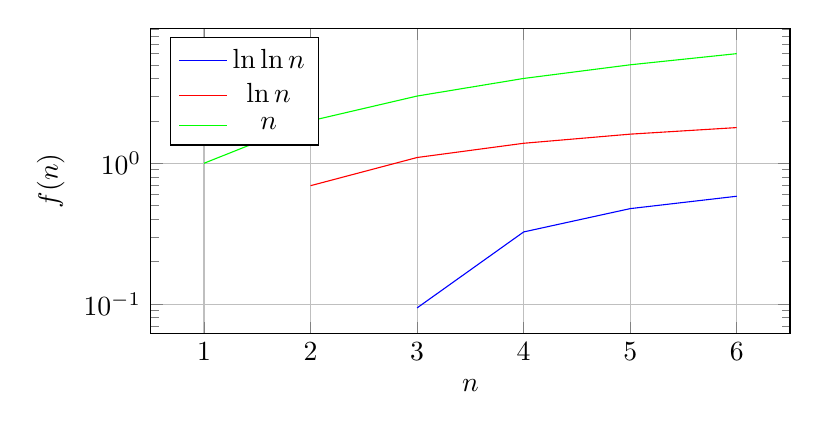
\begin{tikzpicture}
  \begin{axis}[
    width=0.8\textwidth, height=0.45\textwidth,
    xlabel={$n$}, ylabel={$f(n)$}, ymode=log,
    grid=major, legend pos=north west
  ]
    \addplot[blue,mark=none] coordinates {(2,-0.3665) (3,0.0940) (4,0.3254) (5,0.4764) (6,0.5832)};
      \addlegendentry{$\ln\ln n$}
    \addplot[red,mark=none] coordinates {(1,0.0000) (2,0.6931) (3,1.0986) (4,1.3863) (5,1.6094) (6,1.7918)};
      \addlegendentry{$\ln n$}
    \addplot[green,mark=none] coordinates {(1,1) (2,2) (3,3) (4,4) (5,5) (6,6)};
      \addlegendentry{$n$}
  \end{axis}
\end{tikzpicture}
\end{center}


\paragraph*{Exercise 2}
For \(f,g,h\colon\mathbb N\to\mathbb R_{\ge0}\), prove:
\[
\begin{aligned}
1.\;&f\in O(f),\\
2.\;&O(c\,f)=O(f)\quad(\forall c>0),\\
3.\;&f(n)\le g(n)\text{ eventually}\implies O(f)\subseteq O(g),\\
4.\;&O(f)\subseteq O(g)\implies O(f+h)\subseteq O(g+h),\\
5.\;&h(n)>0\;\forall n,\;O(f)\subseteq O(g)\implies O(f\,h)\subseteq O(g\,h).
\end{aligned}
\]
\textbf{Proof.}
\begin{enumerate}[label=\arabic*.]
  \item \(f(n)\le1\cdot f(n)\), so \(f\in O(f)\).
  \item If \(u\in O(c\,f)\), then \(u(n)\le C\,c\,f(n)\), hence \(u\in O(f)\).  Conversely similarly.
  \item If \(f(n)\le g(n)\) for large \(n\) and \(u\in O(f)\), then \(u(n)\le C\,f(n)\le C\,g(n)\), so \(u\in O(g)\).
  \item If \(u\in O(f)\), then \(u(n)+h(n)\le C\,f(n)+h(n)\le C\bigl(f(n)+h(n)\bigr)\), giving \(u+h\in O(f+h)\subseteq O(g+h)\).
  \item If \(u\in O(f)\) and \(h(n)>0\), then \(u(n)\,h(n)\le C\,f(n)\,h(n)\), so \(u\,h\in O(f\,h)\subseteq O(g\,h)\).
\end{enumerate}

\paragraph*{Exercise 3}
Let \(i,j,k,n\in\mathbb N\). Prove:
\[
\begin{aligned}
1.\;&j\le k\implies O(n^j)\subseteq O(n^k),\\
2.\;&j\le k\implies O(n^j+n^k)\subseteq O(n^k),\\
3.\;&O\Bigl(\sum_{m=0}^k a_m\,n^m\Bigr)=O(n^k),\\
4.\;&O(\log n)\subseteq O(n),\\
5.\;&O(n\log n)\subseteq O(n^2).
\end{aligned}
\]

\newpage

\textbf{Proof.}
\begin{enumerate}[label=\arabic*.]
  \item \(n^j\le n^k\) for \(n\ge1\), so \(O(n^j)\subseteq O(n^k)\).
  \item For \(n\ge1\), \(n^j+n^k\le2n^k\), giving \(O(n^j+n^k)\subseteq O(n^k)\).
  \item \(\sum_{m=0}^k a_m n^m\le \bigl(\sum|a_m|\bigr)n^k\).
  \item For \(n\ge2\), \(\log n\le n\).
  \item For \(n\ge2\), \(n\log n\le n^2\).
\end{enumerate}

\paragraph*{Exercise 4}
Which relationships hold between:
\[
\begin{aligned}
1.\;&O(n)\text{ vs.\ }O(\sqrt n),\\
2.\;&O(n^2)\text{ vs.\ }O(2^n),\\
3.\;&O(\log n)\text{ vs.\ }O((\log n)^2),\\
4.\;&O(2^n)\text{ vs.\ }O(3^n),\\
5.\;&O(\log_2n)\text{ vs.\ }O(\log_3n).
\end{aligned}
\]
\textbf{Answer.}
\begin{enumerate}[label=\arabic*.]
  \item \(O(\sqrt n)\subsetneq O(n)\).
  \item \(O(n^2)\subsetneq O(2^n)\).
  \item \(O(\log n)\subseteq O((\log n)^2)\).
  \item \(O(2^n)\subsetneq O(3^n)\).
  \item \(O(\log_2n)=O(\log_3n)\).
\end{enumerate}

\paragraph*{Exercise 5}
Classic sorting comparisons:
\[
\text{bubble sort vs.\ insertion sort},\quad
\text{insertion sort vs.\ merge sort},\quad
\text{merge sort vs.\ quick sort}.
\]
\textbf{Discussion.}
\begin{itemize}
  \item \textbf{Bubble vs.\ Insertion:} Both worst-case \(O(n^2)\), but insertion sort is \(O(n)\) on nearly-sorted input.
  \item \textbf{Insertion vs.\ Merge:} Insertion sort worst-case \(O(n^2)\), merge sort always \(O(n\log n)\).
  \item \textbf{Merge vs.\ Quick:} Merge sort is \(O(n\log n)\) always; quick sort is \(O(n\log n)\) average, \(O(n^2)\) worst, but often faster in practice.
\end{itemize}

\subsubsection{Conclusion}
We’ve surveyed P vs.\ NP, NP-completeness via SAT, practiced ordering and relating functions by asymptotic growth, and applied these insights to sorting algorithms. The included plots illustrate constant-factor and growth-rate comparisons without overwhelming the presentation.

\textbf{Question:} What’s the fastest known quantum sorting algorithm in the query (comparison) model, and how close is it to being practical?

\subsection{Weeks 10 \& 11: Intractable Problems}

\subsubsection{Introduction}
In Weeks 10 and 11 we shift our focus to computational intractability by defining the classes P and NP and the concept of polynomial‐time reductions (Chapter 10.1), proving the NP‐completeness of SAT via Cook’s Theorem (Chapter 10.2), and then applying these ideas through exercises in rewriting formulas into CNF, deciding small SAT instances, and encoding complex constraints like Sudoku into conjunctive normal form.

\subsubsection{Readings}

\paragraph*{Chapter 10.1: The Classes \(\mathrm{P}\) and \(\mathrm{NP}\)}  
We refine decidability to \emph{tractability}.  A language \(L\) is in
\(\mathrm{P}\) if some deterministic TM decides it in time \(O(n^k)\).  A
language \(L\) is in \(\mathrm{NP}\) if some nondeterministic TM accepts
it in time \(O(n^k)\).  We introduce \emph{polynomial–time reductions}—
transformations computable in polynomial time—and define \emph{NP‐completeness}:

\begin{definition}
A language \(L\) is \emph{NP‐complete} if
\begin{enumerate}
  \item \(L\in\mathrm{NP}\), and
  \item for every \(L'\in\mathrm{NP}\), there is a polynomial‐time reduction
    \(L'\le_p L\).
\end{enumerate}
\end{definition}

\paragraph*{Chapter 10.2: SAT and NP‐Completeness}\label{sec:chapter10.2}
\paragraph{The SAT Problem.}  Boolean formulas are built from variables,
\(\land,\lor,\lnot\), and parentheses.  A formula is \emph{satisfiable} if
some assignment of \(\{\mathrm{TRUE},\mathrm{FALSE}\}\) makes it true.
The language
\[
  \mathrm{SAT}
  \;=\;
  \bigl\{\varphi\mid \varphi\text{ a satisfiable Boolean formula}\bigr\}
\]
is in \(\mathrm{NP}\) (guess an assignment, evaluate in polynomial time).
\paragraph{Cook’s Theorem.}  Every \(L\in\mathrm{NP}\) reduces to SAT in
polynomial time; hence SAT is NP‐complete.

\subsubsection{Homework}\label{sec:week8-9-exercises}

\paragraph*{Exercise 1: Rewriting in CNF}  
Rewrite each formula into an equivalent conjunctive normal form.

\[
\varphi_1 := \neg\bigl((a\land b)\;\lor\;(\neg c\land d)\bigr),
\quad
\varphi_2 := \neg\bigl((p\lor q)\to(r\land\neg s)\bigr).
\]

\paragraph{Solution.}
\[
\begin{aligned}
\varphi_1 
&= \neg\bigl(X\lor Y\bigr)
  &&\text{where }X=(a\land b),\;Y=(\neg c\land d)\\
&= \neg X\;\land\;\neg Y\\
&= (\neg a\;\lor\;\neg b)\;\land\;(c\;\lor\;\neg d).
\\[6pt]
\varphi_2 
&= \neg\Bigl(\neg(p\lor q)\;\lor\;(r\land\neg s)\Bigr)
  &&\bigl(P\to Q\equiv\neg P\lor Q\bigr)\\
&= \neg\bigl(\neg X\;\lor\;Y\bigr)
  &&\text{where }X=(p\lor q),\;Y=(r\land\neg s)\\
&= X\;\land\;\neg Y\\
&= (p\lor q)\;\land\;(\neg r\lor s).
\end{aligned}
\]

\paragraph*{Exercise 2: Satisfiability}  
For each formula, decide whether it is satisfiable.  If yes, give a satisfying
assignment; if not, prove no such assignment exists.

\[
\begin{aligned}
\psi_1 &:= (a\lor\neg b)\;\land\;(\neg a\lor b)\;\land\;(\neg a\lor\neg b),\\
\psi_2 &:= (\neg p\lor q)\;\land\;(\neg q\lor r)\;\land\;\neg(\neg p\lor r),\\
\psi_3 &:= (x\lor y)\;\land\;(\neg x\lor y)\;\land\;(x\lor\neg y)\;\land\;(\neg x\lor\neg y).
\end{aligned}
\]

\paragraph{Solution.}
\begin{itemize}
  \item \(\psi_1\): take \(a=\mathrm{FALSE},\,b=\mathrm{FALSE}\).  Then
  \[
    (0\lor1)\land(1\lor0)\land(1\lor1)
    =1\land1\land1=1.
  \]
  Hence \(\psi_1\) is satisfiable.

  \item \(\psi_2\): note
  \[
    \neg(\neg p\lor r)\equiv(p\land\neg r).
  \]
  So \(\psi_2\equiv(\neg p\lor q)\land(\neg q\lor r)\land p\land\neg r\).
  From \(p\) and \(\neg r\) we get \(q\) by the first clause, but then
  \(\neg q\lor r\) becomes \(0\), contradiction.  Thus \(\psi_2\) is
  unsatisfiable.

  \item \(\psi_3\): one checks all four assignments to \((x,y)\) and finds
  each violates some clause.  Hence \(\psi_3\) is unsatisfiable.
\end{itemize}

\paragraph*{Exercise 3: Sudoku CNF Encoding}  
We have boolean variables
\[
  x_{r,c,v},\quad
  r,c,v\in\{1,\dots,9\},
\]
true exactly when cell \((r,c)\) holds value \(v\).  The CNF is
\(\bigwedge_{k=1}^6 C_k\), where:

\[
\begin{aligned}
C_1{:}&\quad
\bigwedge_{r=1}^9\;\bigwedge_{c=1}^9\;\bigl(\,x_{r,c,1}\lor x_{r,c,2}\lor\cdots\lor x_{r,c,9}\bigr),
&&\text{(each cell has at least one value)}\\
C_2{:}&\quad
\bigwedge_{r=1}^9\;\bigwedge_{c=1}^9\;\bigwedge_{\substack{v,w=1\\v\neq w}}^9
\neg\bigl(x_{r,c,v}\land x_{r,c,w}\bigr),
&&\text{(each cell has at most one value)}\\
C_3{:}&\quad
\bigwedge_{r=1}^9\;\bigwedge_{v=1}^9\;\bigl(\,x_{r,1,v}\lor\cdots\lor x_{r,9,v}\bigr),
&&\text{(each row contains each value)}\\
C_4{:}&\quad
\bigwedge_{c=1}^9\;\bigwedge_{v=1}^9\;\bigl(\,x_{1,c,v}\lor\cdots\lor x_{9,c,v}\bigr),
&&\text{(each column contains each value)}\\
C_5{:}&\quad
\bigwedge_{b_r=0}^2\;\bigwedge_{b_c=0}^2\;\bigwedge_{v=1}^9
\;\bigl(x_{3b_r+1,\,3b_c+1,\,v}\;\lor\;\cdots\;\lor\;x_{3b_r+3,\,3b_c+3,\,v}\bigr),
&&\text{(each \(3\times3\) block has each value)}\\
C_6{:}&\quad
\bigwedge_{(r,c)\in\mathrm{Clues}}x_{r,c,v_{r,c}},
&&\text{(respect the given clues).}
\end{aligned}
\]

\subsubsection{Conclusion}
Weeks 8 \& 9 introduced the classes \(\mathrm{P}\) and \(\mathrm{NP}\), the
notion of polynomial–time reduction, and NP‐completeness.  Cook’s Theorem
places SAT at the heart of intractability.  We practiced CNF rewriting,
satisfiability proofs, and large‐scale CNF encodings (Sudoku), reinforcing
both the theoretical limits and the practical modeling power of SAT.
\textbf{Interesting Question}
Is there a practical sub-exponential algorithm for SAT on random formulas,
and how does it relate to the worst-case NP-completeness barrier?

\subsection{Weeks 12 \& 13: Graph Theory}

\subsubsection{Introduction}
During these two weeks we pivot from abstract graph notions to their most celebrated applications in decision-science.  Chapter 14 of Deo is our guide: it begins with transport networks and the classic \emph{max-flow / min-cut} duality, then systematically injects the complications that arise in practice—multiple sources and sinks, vertex capacities, bidirectional (undirected) lines, mandatory lower-bound throughputs, and lossy transmission.  The chapter culminates in two optimisation mainstays: obtaining the cheapest way to ship a required amount (the transportation problem) and orchestrating several commodities that must share the same network (multicommodity flow).  At each stage Deo emphasises fast combinatorial algorithms and explains why they can outperform general linear-programming approaches. \cite{Deo}

\subsubsection{Readings}

\paragraph*{\textbf{14.1} Transport Networks}
subsection 14.1 introduces \emph{transport networks}—weighted directed graphs whose edge capacities model the maximum rate at which a commodity can move between facilities.  A \textbf{flow} assigns non-negative amounts to edges while conserving quantity at every intermediate vertex and achieving value \(w\) from a unique source \(s\) to sink \(t\).  Deo formalises the \emph{maximal-flow} problem, sketches the linear-programming formulation, and then proves the \textbf{Max-Flow Min-Cut Theorem}: the greatest achievable flow equals the minimum capacity of any \(s\!-\!t\) cut.  A constructive proof underlies the classic augmenting-path algorithm that iteratively raises the flow until no augmenting path remains. \cite{Deo}

\paragraph*{\textbf{14.2} Extensions of Max-Flow Min-Cut}
subsection 14.2 generalises the basic theorem to more complex networks.  
\begin{itemize}[nosep]
  \item \emph{Multiple sources/sinks}: a supersource and supersink convert the instance to the single-commodity case, unless each source must reach a particular sink (the multicommodity variant).  
  \item \emph{Vertex capacities}: split a capacitated vertex into an in-vertex and out-vertex linked by an edge whose capacity equals the vertex limit.  
  \item \emph{Undirected edges}: replace each undirected edge by two opposite directed edges that share the same capacity.  
  \item \emph{Lower bounds}: allow each edge to require at least \(b_{ij}\) units of flow and derive feasibility/optimality conditions in terms of modified cuts.  
  \item \emph{Lossy networks}: assign an efficiency factor \(\lambda_{ij}\) so the out-flow equals \(\lambda_{ij}\) times the in-flow; analogous optimal-flow results hold.  
\end{itemize}
These adaptations preserve the cut-flow duality or indicate when additional constraints break it. \cite{Deo}

\paragraph*{\textbf{14.3} Minimal-Cost Flows}
subsection 14.3 attaches a per-unit cost \(d_{ij}\) to every edge and asks for the cheapest flow of prescribed value \(w\).  Deo connects this \emph{transportation problem} with linear programming but emphasises a combinatorial solution: iteratively send flow along the least-cost \emph{unsaturated} \(s\!-\!t\) path, where path cost counts forward-edge expenses minus backward-edge savings.  A key optimality lemma shows that augmenting by the cheapest unsaturated path always preserves minimality; the process terminates when no such path exists, yielding a minimal-cost maximal flow. \cite{Deo}

\paragraph*{\textbf{14.4} Multicommodity Flow}
subsection 14.4 tackles networks that simultaneously carry \(k\) distinct commodities, each with its own source and sink but sharing edge capacities.  Edge constraints become \(\sum_{m=1}^{k}f_{ij}^{(m)} \le c_{ij}\), and flow conservation holds for every commodity.  The chapter highlights two fundamental tasks: (i) maximise the \emph{total} shipped amount \(\sum_{m}w_m\) and (ii) decide feasibility for specified \((w_1,\dots,w_k)\).  Unlike the single-commodity case, no simple cut characterisation exists in general—only special settings (e.g.\ two commodities in an undirected graph) admit a max-flow min-cut analogue.  The discussion underscores the added complexity that competition for capacity introduces. \cite{Deo}

\newpage

\subsubsection{Exercises}
\paragraph*{Exercise 1 (Max-flow \& minimal-cut)}

\paragraph{Network description.}
The directed graph has source \(s\) and sink \(t\) with capacities shown as
“flow / capacity”:

\[
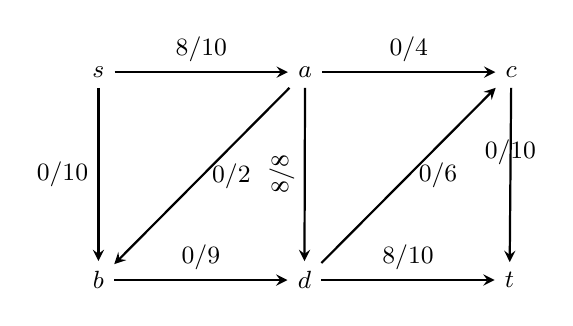
\begin{tikzpicture}[
    node distance=22mm, >=stealth, thick,
    every node/.style={font=\small}
]
\node (s) {$s$};
\node[right=of s] (a) {$a$};
\node[below=of s] (b) {$b$};
\node[right=of a] (c) {$c$};
\node[right=of b] (d) {$d$};
\node[right=of d] (t) {$t$};

\path[->]
 (s) edge node[above] {$8/10$} (a)
      edge node[left]  {$0/10$} (b)
 (a) edge node[right] {$0/2$}  (b)
      edge node[above] {$0/4$} (c)
      edge node[sloped,above] {$8/8$}  (d)
 (b) edge node[above] {$0/9$}  (d)
 (d) edge[left] node[right] {$0/6$} (c)
      edge node[above] {$8/10$} (t)
 (c) edge node[above] {$0/10$} (t);
\end{tikzpicture}
\]

The initial flow has value \(8\).

\paragraph{(1) Ford–Fulkerson augmentation.}
\begin{enumerate}[label=\arabic*. ,leftmargin=2.3em]
  \item Residual path \(s\!\to b\!\to d\!\to t\)  
        \(\min\) residual = 2  
        \(\Rightarrow\) add 2.
  \item Residual path \(s\!\to b\!\to d\!\to c\!\to t\)  
        \(\min\) residual = 6  
        \(\Rightarrow\) add 6.
  \item Residual path \(s\!\to a\!\to c\!\to t\)  
        \(\min\) residual = 2  
        \(\Rightarrow\) add 2.
  \item Residual path \(s\!\to b\!\to d\!\to a\!\to c\!\to t\)  
        \(\min\) residual = 1  
        \(\Rightarrow\) add 1.
\end{enumerate}

No further \(s\!-\!t\) path exists in the residual graph, so the algorithm
terminates with

\[
\boxed{\text{maximum flow value }=19}.
\]

The resulting flow on each edge is

\[
\begin{array}{c|c@{\;\;}c}
\text{edge} & \text{flow}/\text{capacity} & \\ \hline
s\to a & 10/10, & s\to b\; 9/10 \\
a\to b & 0/2,   & a\to c\; 3/4,\; a\to d\; 7/8 \\
b\to d & 9/9,   & d\to c\; 6/6,\; d\to t\; 10/10,\; c\to t\; 9/10
\end{array}
\]

\paragraph{(2) Minimal \(s\text{–}t\) cut.}
Vertices reachable from \(s\) in the final residual graph are
\(P=\{s,b\}\).
Edges leaving \(P\) are \(s\to a\;(10)\) and \(b\to d\;(9)\);
their total capacity is
\[
c(P,\bar P)=10+9=19,
\]
which equals the maximum-flow value, so \((P,\bar P)\) is a minimal cut.

\paragraph{(3) Uniqueness of a maximal flow.}
A maximum-flow \emph{value} is unique, but the \emph{flow pattern} need not
be—different distributions on parallel augmenting paths can yield the same
value.  In this network, for example, one may shift up to one unit from the
path \(s\to a\to d\to t\) to \(s\to a\to c\to t\) (while respecting
capacities) and still obtain value 19.

\newpage

\paragraph*{Exercise 2 (An unknown algorithm)}

\paragraph{Algorithm.}
\begin{lstlisting}
  fun unknown(n)
  1. r := 0
  2. for k := 1 to n-1 do
  3.     for l := k+1 to n do
  4.         for m := 1 to l do
  5.             r := r + 1
  6. return r
\end{lstlisting}  

\paragraph{1) Returned value as a function of \(n\).}
The innermost statement (line 5) executes once for every triple
\((k,l,m)\) that satisfies
\[
1\le k\le n-1,\qquad k+1\le l\le n,\qquad 1\le m\le l .
\]
Hence
\[
r(n)=\sum_{k=1}^{n-1}\;\sum_{l=k+1}^{n}\;\sum_{m=1}^{l}1
      =\sum_{k=1}^{n-1}\;\sum_{l=k+1}^{n} l .
\]
Fix \(l\).  It appears in the inner sum whenever \(k<l\), i.e.\ for
\(k=1,2,\dots,l-1\) (a total of \(l-1\) choices).  Therefore
\[
r(n)=\sum_{l=2}^{n} l(l-1)
     =\sum_{l=1}^{n} (l^{2}-l)
     =\Bigl(\sum_{l=1}^{n} l^{2}\Bigr)-\Bigl(\sum_{l=1}^{n} l\Bigr).
\]
Using the given formulas
\(
\sum_{i=1}^{n} i = \tfrac{n(n+1)}{2}
\)
and
\(
\sum_{i=1}^{n} i^{2}= \tfrac{n(n+1)(2n+1)}{6},
\)
we obtain
\[
r(n)=\frac{n(n+1)(2n+1)}{6}-\frac{n(n+1)}{2}
     =\frac{n(n+1)(2n-2)}{6}
     =\boxed{\dfrac{n(n+1)(n-1)}{3}}.
\]

\paragraph{2) Worst-case running time (Big-O).}
The algorithm performs \(\Theta\!\bigl(r(n)\bigr)\) basic operations.
Since
\[
r(n)=\frac{n(n+1)(n-1)}{3}
     =\frac{1}{3}n^{3}+O(n^{2}),
\]
the worst-case running time grows on the order of \(n^{3}\):
\[
\boxed{T_{\text{worst}}(n)=O(n^{3}).}
\]

\newpage

\section{Synthesis}

Looking back over the entire semester of CPSC-406, I see how the individual topics we covered—from finite automata and formal languages to undecidability, complexity theory, and finally, graph algorithms—have gradually formed a cohesive and comprehensive understanding of algorithm analysis. At first, the course started straightforwardly enough, reviewing concepts like deterministic finite automata (DFAs) and nondeterministic finite automata (NFAs). Even though I'd seen some of these ideas before in previous coursework, writing them up formally forced me to pay closer attention to small details I'd previously overlooked. In particular, the precise definition of transitions, accepting states, and formal languages became clearer as I structured these ideas in LaTeX. 

The transition from finite automata to Turing machines marked a significant step. Initially, Turing machines seemed unnecessarily complex compared to DFAs and NFAs. However, through exercises where we explicitly constructed and simulated these machines, it became clear why Turing machines are foundational in computer science. Their ability to capture all computable functions—while still being relatively simple—demonstrated clearly why they're the standard for formalizing the concept of computability. The Halting Problem was an especially critical moment for my understanding. At first, the idea of an undecidable problem felt abstract, but the clarity of the proof made a deep impression. I recognized how natural and fundamental this limitation was. Attempting to understand precisely why certain problems defy algorithmic solutions was challenging, yet it solidified my grasp of what "decidable" really means in practice.

The classes P, NP, and NP-complete initially felt abstract, but exploring concrete examples—particularly through Boolean satisfiability (SAT)—helped ground my understanding. I found Cook's theorem particularly insightful, especially the idea that SAT could encapsulate every other NP problem. The significance of polynomial-time reductions was somewhat vague until I actively applied them to real examples, such as encoding Sudoku puzzles into CNF. This exercise was both enjoyable and enlightening, highlighting the deep connections between theoretical complexity classes and real-world applications.

Moreover, comparing different complexity classes—like understanding why NP-complete problems are considered practically difficult—was fascinating. It emphasized the value of understanding the theoretical limits when working on real computational problems. Sorting algorithms, too, provided a valuable practical connection. Analyzing and comparing algorithmic runtimes through Big-O notation and asymptotic analysis showed me clearly how theory and practice intersect. Problems that seemed trivially solvable became significantly more interesting when viewed through the lens of efficiency and scalability.

Graph algorithms further solidified this link between theory and real-world utility. Concepts like maximum flow, minimum cut, and their variants appeared immediately practical and applicable. Working through these examples in detail, particularly with the Ford–Fulkerson algorithm, helped clarify concepts that had felt abstract earlier. It was satisfying to see how theoretical efficiency measures directly impact their practical feasibility in applications like network routing and optimization. 

One of the most challenging aspects of the course was maintaining a sense of continuity between topics that initially appeared disconnected. However, as I synthesized these topics week by week, I realized how each concept naturally built on the previous one. The structured note-taking and reflection process provided essential scaffolding, enabling me to make connections that might otherwise have gone unnoticed. I was particularly struck by how seemingly unrelated theoretical concepts from automata theory to complexity theory, all fed into the broader goal of understanding algorithmic behavior and limitations.

Overall, the synthesis of my learning this semester was significantly shaped by actively engaging with the course material through regular writing, reflecting, and problem-solving. The combined effort of understanding theory, practicing problem-solving, and clearly communicating my ideas has not only strengthened my foundational knowledge but also prepared me to better approach complex algorithmic problems in future coursework, research, or industry work. This experience underscored the value of clearly articulating complex ideas, reinforcing the idea that deep understanding arises not only from reading and problem-solving but also from careful reflection and communication.


\section{Evidence Of Participation}
\subsection*{1. Quantum Uncertainty and Scientific Limits — Guest Lecture Reflection}

I found the recent lecture at Chapman University very stimulating. Reflecting on the inherent limits of the scientific method generates a unique sense of existential contemplation. As someone who identifies philosophically with absurdist nihilism, confronting the boundary of scientific knowledge evokes both curiosity and an odd sense of existential dread. When I was younger, I firmly believed in a fully deterministic universe—a universe complex, yet entirely quantifiable. In this deterministic worldview, knowing the complete initial conditions of the universe would, in theory, allow one to predict with absolute certainty every future event. Under such assumptions, science appears concrete and fully capable of unveiling reality. However, quantum mechanics profoundly disrupts this clear-cut vision of reality.

Over the past year, my studies at Chapman in quantum mechanics have consistently challenged and reshaped my understanding. The concept of quantum uncertainty is particularly perplexing when applied to large, chaotic ensembles of particles. Examples of such systems include Saturn’s moon Hyperion, Earth's oceans, or even individual humans. These systems, due to their chaotic nature, exhibit a profoundly uncertain and indeterminate future when considered through the lens of quantum mechanics. This probabilistic perspective aligns interestingly with my understanding of the de Broglie wavelength associated with every physical object.

According to quantum theory, each object possesses an associated wavelength, defined as Planck's constant divided by the object's momentum. Given that Planck's constant is extremely small—on the order of \(10^{-34}\)—it becomes clear why macroscopic, fast-moving objects exhibit incredibly short wavelengths. Consequently, the quantum wave packets representing larger objects like humans appear sharply defined, with positions and momenta that seem essentially certain. Although strictly speaking every object, including humans, has a wavefunction, their macroscopic scale makes quantum wavelike behavior practically negligible. For instance, this negligible quantum behavior is why humans don't visibly diffract when passing through doorways. A simple calculation illustrates this clearly: a 70\,kg human moving at 1\,m/s through a 1\,m-wide doorway yields a diffraction angle of roughly \(10^{-35}\) radians. Even at a distance of one full light-year from the doorway, the separation between the first and second-order diffraction fringes would only be around \(10^{-15}\,m\), significantly smaller than atomic scales. Hence, we observe no practical diffraction effects.

The implications of the de Broglie wavelength are also fundamental to Bohr’s atomic model. In Bohr’s model of the hydrogen atom, the valid electron radii and energy levels arise because electrons must form standing waves. Only radii corresponding to integer multiples of the electron’s de Broglie wavelength allow for continuous wavefunctions; otherwise, the electron’s wavefunction would exhibit discontinuities. Interestingly, attempting to apply this same logic to macroscopic systems like celestial orbits highlights important distinctions. For example, the Moon's de Broglie wavelength, given its enormous mass and velocity, is approximately \(10^{-61}\,m\). This scale is far smaller even than the Planck length—the shortest meaningful length scale in physics—so quantum constraints like standing wave conditions effectively become meaningless, allowing the Moon to occupy orbits that appear continuous.

Despite this, the Moon still behaves as a quantum wave packet, albeit at an unobservable scale. This observation does not violate the Heisenberg uncertainty principle, since the Moon’s momentum is so large that the product of uncertainties in position and momentum easily surpasses the fundamental quantum limit. Additionally, unlike Hyperion, the Moon's relatively stable orbit is less chaotic, meaning quantum uncertainties have minimal influence on its future position predictions. Less chaotic systems, in general, are less sensitive to small errors in initial conditions, resulting in more predictable trajectories.

Considering these concepts, it is fascinating (although likely flawed in certain assumptions) to contemplate the quantum effects on macroscopic celestial systems. In particular, the lecturer's mention of Hyperion intrigued me greatly. I am curious how quantum uncertainty was quantitatively incorporated into the calculations that predicted the breakdown of classical predictability within approximately 50 years. Understanding the exact methodology and assumptions involved would be enlightening and could further clarify the subtle interplay between quantum mechanics and chaotic macroscopic systems.

\subsection*{2. Video Summary – Grover's Algorithm and Quantum Speedup}

In this video\footnote{\url{https://www.youtube.com/watch?v=RQWpF2Gb-gU&t=798s}}, the narrator critically examines common misconceptions surrounding quantum computing, particularly the oversimplified notion that quantum computers simply evaluate all possible bit sequences simultaneously via superposition. Using a quiz to highlight misunderstandings, the speaker demonstrates that while this notion gestures toward reality, it misleadingly inflates expectations. The discussion centers on a classic search problem—finding a unique input that causes a function to return true—and compares the runtime between classical and quantum approaches. Classically, the task scales linearly with input size \(O(n)\), but quantumly, Grover's algorithm enables a square root speedup to \(O(\sqrt{n})\). This represents a meaningful, though not exponential, improvement, and it is applicable to a broad class of verifiable problems known as NP.

The video builds from foundational concepts—like state vectors, qubits, and probability amplitudes—to a full geometric walkthrough of Grover's algorithm. It emphasizes that quantum computation operates not on visible parallelism, but on coherent manipulations of state vectors in high-dimensional Hilbert spaces. The real speedup arises not from evaluating all inputs at once, but from leveraging quantum reflections and interference to iteratively concentrate amplitude onto the correct output. Ultimately, the video frames quantum speedup as a kind of diagonal shortcut through a state space—a geometrically elegant and mathematically bounded detour—rather than an omnipotent parallelism. It closes with a reflection on pedagogy and analogy, including a comparison to a classical $\pi$-computing block collision problem, further grounding abstract quantum behavior in intuitive physics-inspired models.

\subsection*{3. Video Summary – Gradient Descent and Neural Networks}

This video introduces gradient descent through the lens of training a simple neural network for digit classification using the MNIST dataset. The process begins with random initialization of over 13,000 weights and biases in a network structured with two hidden layers. The network initially performs poorly, producing output activations that don't align with the correct labels. To correct this, a cost function is defined, measuring the error between the output and the desired result by summing the squared differences across all output neurons. The average cost over thousands of training examples becomes the metric of the network’s performance. Gradient descent is used to reduce this cost: by computing the slope of the cost function with respect to each parameter, the network updates its weights and biases in the direction that most quickly decreases the cost. This iterative approach, driven by backpropagation (to be discussed in a later video), forms the mathematical core of how the network "learns" by minimizing its error over time.

Throughout the video, the visual metaphor of a ball rolling down a hill is used to explain descent in both single-variable and multivariable functions. Each component of the gradient vector reflects both the direction and relative importance of adjusting each parameter. In practice, some weights have a much larger impact on classification accuracy than others, and gradient descent captures this. The video also touches on limitations: the cost landscape has many local minima, and the solution found depends on the starting point. Despite this, the basic network described achieves about 96\% classification accuracy, with performance improving to 98\% with minor tweaks. However, analysis of hidden layers reveals that the learned features aren’t always intuitive—suggesting the network may succeed through memorization rather than generalized pattern recognition. This raises questions about structure, generalization, and overfitting in deep learning systems.\footnote{\url{https://www.youtube.com/watch?v=IHZwWFHWa-w}}

\newpage

\subsection*{4. Video Summary – Hash Algorithms and File Verification}

This video introduces hash algorithms and their role in verifying data integrity during file transfers. The concept is compared to the check digit on barcodes or credit cards, which acts as a quick check against user error. Hash algorithms extend this concept to entire files, producing a fixed-length hexadecimal string—essentially a signature that summarizes the entire file’s contents. Although it's computationally impossible to reverse a hash back to the original data, any change in the original file (even a single bit) results in a completely different hash—this property is known as the avalanche effect. Three main criteria for a good hash algorithm are identified: speed, sensitivity to small changes, and resistance to hash collisions (cases where different files produce the same hash). The video illustrates that while naturally occurring collisions are mathematically inevitable due to the pigeonhole principle, the real threat is in engineered collisions, which could be used to falsify documents while maintaining the same hash.

The video also explores real-world implications of broken hash functions. MD5, once a widely used algorithm, is now obsolete due to known vulnerabilities and hash collisions. Because it was so commonly used, and many hashes are indexed by search engines, it is trivial to reverse MD5 hashes in some cases—making it especially inappropriate for password storage. Even SHA-1, which replaced MD5, is now considered insecure due to the increasing computational power available. SHA-2 is currently the widely accepted standard, with SHA-3 being phased in. The video cautions against common misuses, like assuming hashes posted on software download sites guarantee security; if a malicious actor has compromised the server, they could alter both the software and the displayed hash. The overarching message emphasizes that while hashes are excellent for verifying integrity, they should not be treated as a full security mechanism.\footnote{\url{https://www.youtube.com/watch?v=b4b8ktEV4Bg}}

\subsection*{5. Video Summary – Cracking Enigma with Modern Methods}

This video revisits the legendary Enigma machine—used by the Germans during World War II—and explores whether modern computers can efficiently break its encryption. While the Enigma's design is mechanical and was incredibly secure for its time, today's computing power invites the question: can it now be brute-forced? The video provides a clear breakdown of how the Enigma machine works: input letters pass through a plugboard, three rotors, a reflector, and back again through the system, resulting in a complex letter substitution that changes with every keystroke. This creates a dynamic cipher that was once infeasible to brute-force due to its vast number of configurations. However, the speaker attempts a ciphertext-only attack by simulating Enigma settings in code and using statistical analysis to identify likely plaintext candidates without any known plaintext assumptions.

The core method used is the index of coincidence (IOC), which quantifies how "English-like" a decrypted output is. English text typically has an IOC of around 0.067, while random strings hover near 0.038. The code tests many rotor combinations and configurations to maximize the IOC of the output, gradually approaching more intelligible plaintext. Once promising rotor configurations are identified, ring settings and plugboard combinations are iteratively optimized. Though this approach cannot crack short messages reliably—due to insufficient data for meaningful statistical patterns—longer messages (1000+ characters) yield more effective results. The final decrypted text is revealed to be a garbled but increasingly accurate version of Alan Turing's famous “Can machines think?” paper. The video concludes that although Enigma is no longer considered secure, it’s not trivial to break without careful strategy. Importantly, unlike Enigma, modern encryption algorithms are resistant to partial-key brute-force attacks and do not degrade gracefully with partial key knowledge.

\newpage

\subsection*{6. Video Summary – Analog Computing and the Future of AI}

This video explores the resurgence of analog computing and its potential role in the future of artificial intelligence. For centuries, analog devices were used to simulate physical systems, from calculating tides to guiding missiles. Today, a perfect storm of challenges facing digital computing—rising energy demands, the Von Neumann bottleneck, and the limitations of Moore’s Law—has renewed interest in analog machines. Unlike digital computers, which operate on binary logic, analog computers represent data as continuous voltages. This allows them to simulate differential equations in real time with far fewer components and much less energy. For instance, analog circuitry can directly solve equations like the Lorenz system by physically modeling them in voltage behavior.

The connection to AI comes from the structure of neural networks, which heavily rely on matrix multiplication. Since analog circuits can multiply and sum values naturally through electrical properties, they are well-suited to AI workloads. Startups like Mythic AI have built analog chips using flash memory cells as variable resistors, enabling energy-efficient inference with neural nets. Though analog systems face issues like imprecision and noise accumulation, hybrid approaches—where analog computation is interleaved with digital processing—offer practical solutions. The video suggests that while digital has dominated computation for decades, the future might lie in combining analog's efficiency with digital's precision, especially for neural network inference. As the boundaries of computation are pushed, analog might become the key to unlocking human-like AI.\footnote{\url{https://www.youtube.com/watch?v=GVsUOuSjvcg}}

\subsection*{7. Video Summary – Building a Minimal Programming Language}

In this video, the creator walks through designing and implementing a miniature programming language from scratch using Python. The language begins as a simple reverse Polish notation (RPN) calculator that evaluates expressions like \texttt{"2 3 +"} by pushing values onto a stack and applying operations. From this basic foundation, the language is gradually expanded to support multi-line inputs, variables, and simple parsing via Python's \texttt{split()} function. The program can read from a file, tokenize each line, and maintain a variable dictionary to track assignments, enabling expressions like \texttt{"x = 2 3 +"} and \texttt{"y = x 5 +"}.

To make the system feel more like a genuine language, the video adds control flow with \texttt{while} loops and comparison operations. Loops are supported by managing a program counter and scanning lines for \texttt{while} and \texttt{end} keywords to handle conditional jumps. The culmination of the language’s expressiveness is demonstrated by implementing the factorial function, showcasing variable mutation and loop-based computation. With just under 40 lines of Python code, the project illustrates how modest components—stack-based evaluation, minimal parsing, and simple control structures—can create a functioning interpreted language, providing insight into how real programming languages are built from fundamental parts.\footnote{\url{https://www.youtube.com/watch?v=fc1ZU80pCCg}}

\subsection*{8. Video Summary – Ethics in AI, not of AI}

In this Topos colloquium, philosopher and data scientist David Danks presents a compelling argument that ethics should not be confined to the deployment stage of AI, but rather integrated into every phase of research and development. Danks rejects the idea that algorithms and mathematical models are ethically neutral, asserting that choices made in problem framing, design constraints, and evaluation criteria are inherently value-laden.

Instead of relying on high-level ethical principles, which often lack actionable guidance, he advocates for practice-oriented approaches—like ethical triage checklists, model documentation tools (e.g., model cards), and value-sensitive design methodologies. These help researchers identify and navigate ethical implications throughout their work. Danks concludes by calling for a cultural shift: ethical awareness should be seen not as an optional virtue, but as an essential component of research competence.

\footnote{\url{https://www.youtube.com/watch?v=kEf_MTqeXWg}}

\subsection*{9. Video Summary – Birthday Paradox \& Hash Collisions}

Mike Pound introduces the birthday paradox to illustrate why hash collisions occur in cryptography. A collision happens when two distinct inputs generate the same hash output. Although hash functions, such as SHA-256, produce extremely large outputs (e.g., \(2^{256}\) possibilities), collisions become statistically probable far sooner than intuition suggests, due to the pigeonhole principle. Mike demonstrates this paradox practically: among 23 people, the probability of a shared birthday is around 50\%, and it jumps to approximately 90\% with 40 people. Such collisions in cryptographic hashes can potentially weaken digital signatures and security protocols. Therefore, contemporary hash functions use significantly longer output lengths (256 bits or more) to mitigate the practical risk of collisions.

\footnote{\url{https://www.youtube.com/watch?v=jsraR-el8_o}}

\subsection*{10. Video Summary – Random Numbers (the next bit)}

James Clewitt explores the concept of randomness, demonstrating that people tend to choose "random" numbers predictably (e.g., many choosing 7). He distinguishes pseudorandom numbers—produced by deterministic computational algorithms—from genuinely random numbers, which stem from inherently unpredictable phenomena like radioactive decay. Clewitt uses radioactive strontium-90 and a Geiger counter to produce truly random numbers, resulting in a Gaussian distribution. He underscores that randomness is not a property of single numbers, but rather the unpredictability inherent in sequences of numbers, comparing human intuition, computational methods, and physical randomness.

\footnote{\url{https://www.youtube.com/watch?v=SxP30euw3-0}}


\section{Conclusion}\label{conclusion}

Throughout CPSC-406: Algorithm Analysis, I have developed a deeper understanding of the foundational principles underlying computation, complexity, and decidability. The course began with finite automata and formal languages, laying a rigorous foundation for algorithmic thinking, and progressed through the complexities of Turing machines, undecidability, NP-completeness, and practical graph-theoretic algorithms. By working systematically through weekly exercises and reflections, I've honed my skills not only in theoretical analysis but also in effectively communicating complex concepts clearly and concisely.

Among the most valuable insights has been the direct applicability of seemingly abstract concepts, such as reducibility and complexity classes, to real-world problems like network flow optimization and satisfiability constraints in computational logic. The structured approach of documenting weekly notes, homework solutions, and explorations allowed me to synthesize my learning progressively, building both depth and breadth across topics.

In terms of improvements, future iterations of the course might benefit from further integrating algorithmic implementation with theory, offering practical coding exercises to reinforce abstract theoretical concepts more concretely. Overall, the course has significantly strengthened my analytical and critical thinking abilities, preparing me to engage more deeply in both academic research and professional software engineering contexts.

\newpage

\section{Bibliography}
\begin{thebibliography}{99}

  \bibitem[HMU]{HMU}
  J.~E.~Hopcroft, R.~Motwani, J.~D.~Ullman:  
  \emph{Introduction to Automata Theory, Languages, and Computation} (3rd ed.).  
  \href{https://archive.org/details/hopcroft-motwani-ullman-introduction-to-automata-theory-languages-and-computations-3rd-edition/page/65/mode/1up?view=theater}{Archive.org Link}.
  
  \bibitem[Deo]{Deo}
  N.~Deo:  
  \emph{Graph Theory with Applications to Engineering and Computer Science}.  
  Prentice-Hall, 1974.  
  \href{https://archive.org/details/GraphTheoryWithApplicationsToEngineeringAndComputerScience/page/n108/mode/1up?view=theater}{Archive.org Link}.
  
  \end{thebibliography}

\end{document}